\documentclass[handout,aspectratio=169]{beamer}
%\usepackage{pgfpages}
%\pgfpagesuselayout{4 on 1}[a4paper,border shrink=5mm]
\usetheme[block=fill,progressbar=frametitle,numbering=none]{metropolis}
\usepackage{animate}
% Paquetes de la ams
\usepackage{amsmath,amsthm,amssymb,amsfonts}
% Codificacion UTF-8
\usepackage[utf8]{inputenc}
% Tablas e imagenes en espaniol
\usepackage[spanish,es-tabla]{babel}
% Mejores graficos
\usepackage{graphicx}
% tablas mas lindas
\usepackage{booktabs}
% Links a urls
\usepackage{url}
% Linkear referencias en pdfs
\usepackage{hyperref}
% Texto mas lindo para los pie de figura
\usepackage[margin=10pt,font=small,labelfont=bf, labelsep=endash]{caption}

% Citas
\usepackage[backend=biber,style=ieee]{biblatex}
\addbibresource{biblio.bib}

% Codigo
\usepackage{listings}

% Dir tree
\usepackage{dirtree}

% Pagina en blanco cuando ha
\usepackage{emptypage}

\definecolor{A11}{HTML}{B2DF8A}
\definecolor{A12}{HTML}{33A02C}
\definecolor{A23}{HTML}{FDBF6F}
\definecolor{A24}{HTML}{FF7F00}
\definecolor{B15}{HTML}{FB9A99}
\definecolor{B16}{HTML}{E31A1C}
\definecolor{B27}{HTML}{A6CEE3}
\definecolor{B28}{HTML}{1F78B4}

% Ejemplos, observaciones y teorema
\theoremstyle{definition}
\newtheorem{exa}{Ejemplo}[section]
\newtheorem*{obs}{Observación}
\newtheorem{que}{Pregunta}[section]
\newtheorem{dex}{Definicion}[section]

\usepackage{multimedia}

\title{Interpretación visual}
\subtitle{Nivel 0}

\author{Marina Compagnucci \and Francisco Nemiña}

\institute{Unidad de Educación y Formación Masiva \\ Comisión Nacional de Actividades Espaciales}

\date{}
\graphicspath{{./figs/}}

\begin{document}

\maketitle

\begin{frame}{Esquema de la presentación}
  \setbeamertemplate{section in toc}[sections numbered]
  \tableofcontents[hideallsubsections]
\end{frame}

\section{La teledetección}
\subsection{Definición}
\begin{frame}{\secname : \subsecname}
    \begin{block}{Definición}
    La teledetección es medir un sistema sin estar en contacto con el. En particular, en el contexto espacial, hablamos de teledetección cuando hablamos de las mediciones de la tierra realizadas por un satélite
    \end{block}
\end{frame}
%--- Next Frame ---%

\begin{frame}{\secname : \subsecname}
    \begin{figure}[h!]
        \centering
        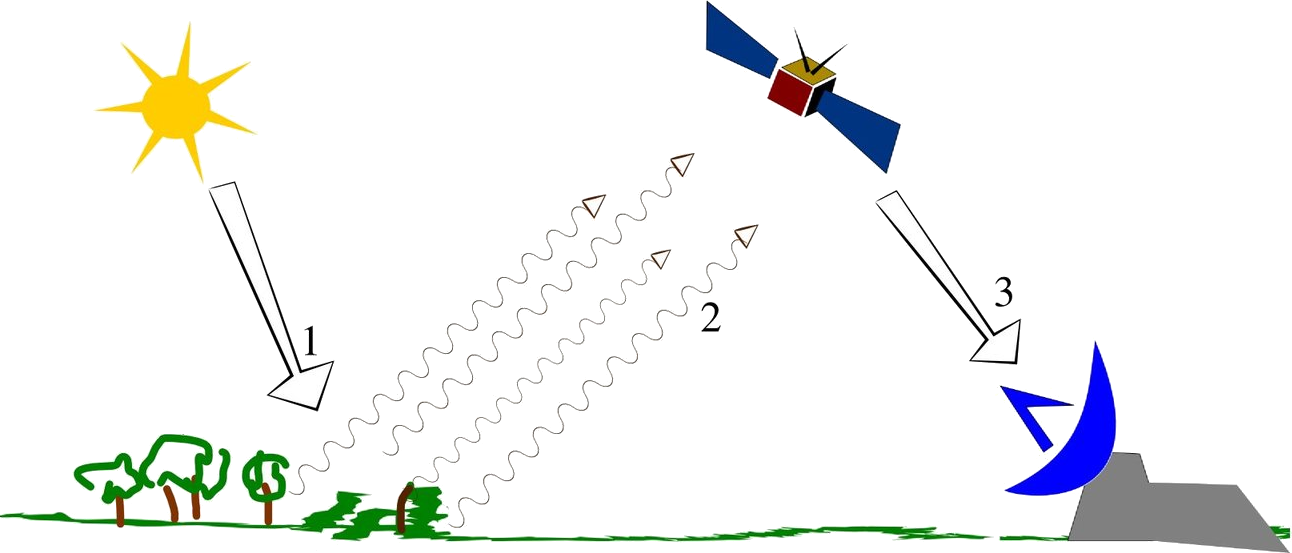
\includegraphics[width=0.9\textwidth]{fig:pasivo.png}
        \caption{Esquema de adquisición de datos para un sensor pasivo. \cite{wiki:rs}}
        \label{fig:pasivo}
    \end{figure}
\end{frame}
%--- Next Frame ---%}

\begin{frame}{\secname : \subsecname}
    \begin{figure}[h!]
        \centering
        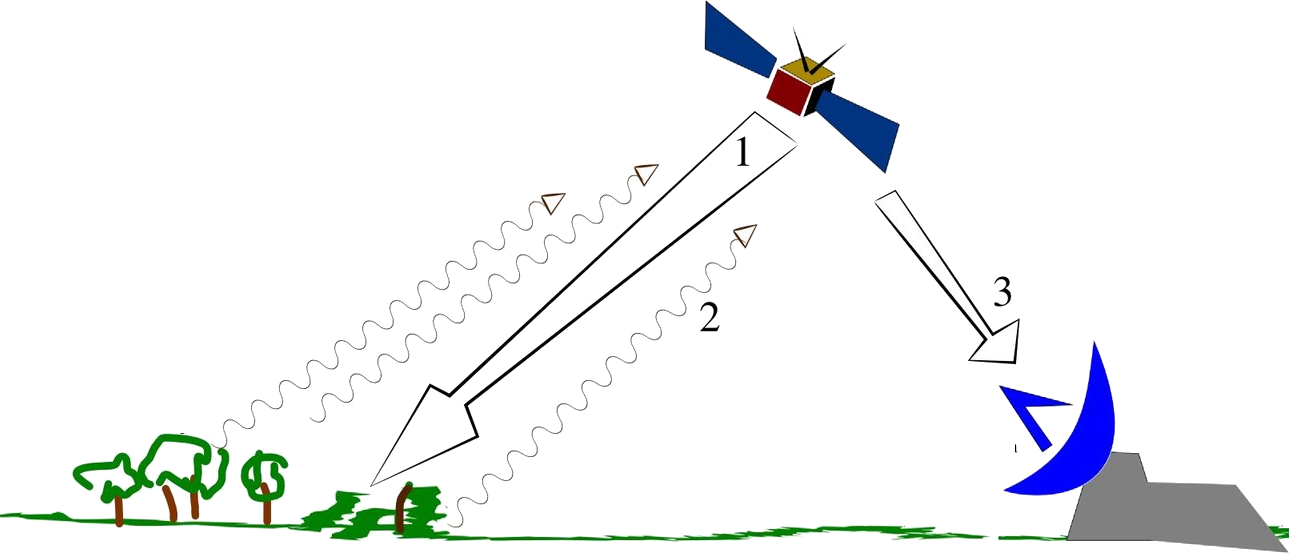
\includegraphics[width=0.9\textwidth]{fig:activo.png}
        \caption{Esquema de adquisición de datos para un sensor activo. \cite{wiki:rs}}
        \label{fig:activo}
    \end{figure}
\end{frame}
%--- Next Frame ---%}

\subsection{Aplicaciones}

\begin{frame}{\secname : \subsecname}
    \begin{exampleblock}{Google Earth}
        \begin{figure}[h!]
            \centering
            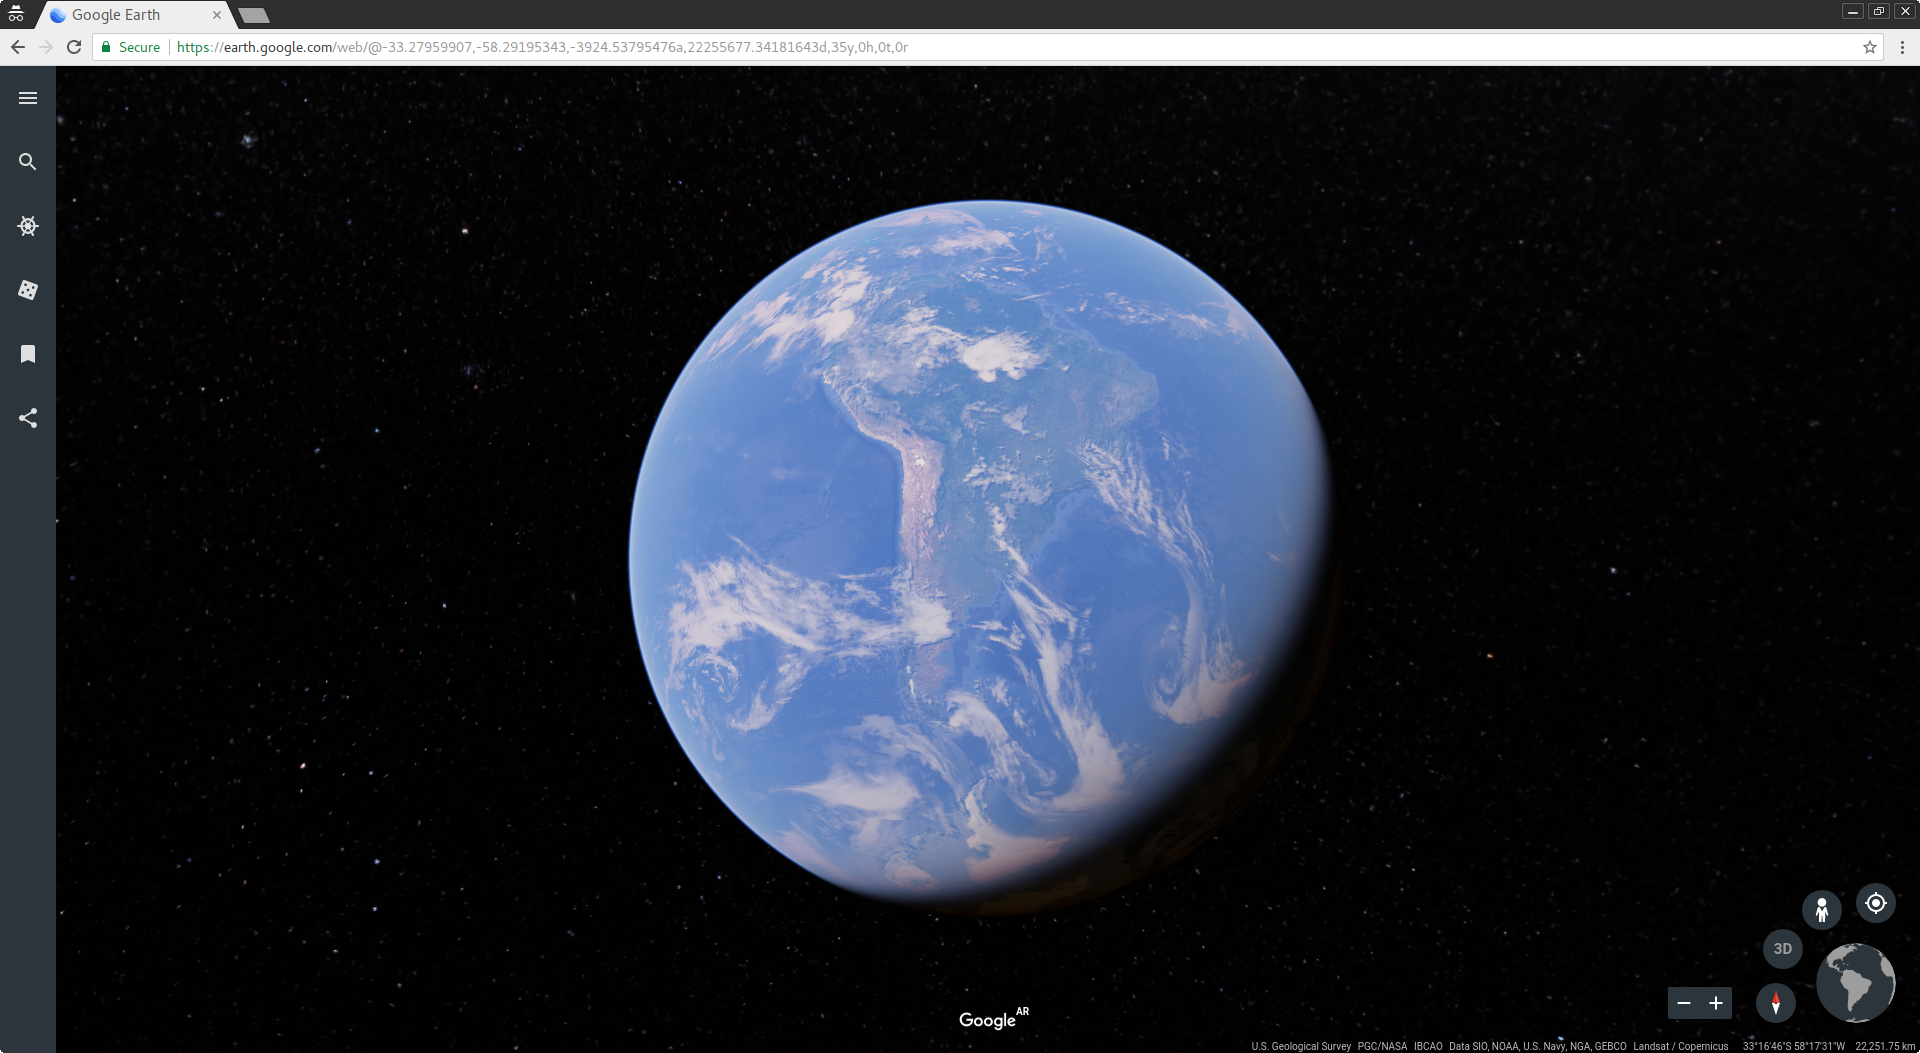
\includegraphics[width=0.75\textwidth]{fig:GE.png}
            \label{fig:GE}
        \end{figure}
    \end{exampleblock}
\end{frame}
%--- Next Frame ---%}

\begin{frame}{\secname : \subsecname}
    \begin{exampleblock}{Mapas de humedad del suelo - SMOS}
        \begin{figure}[h!]
            \centering
            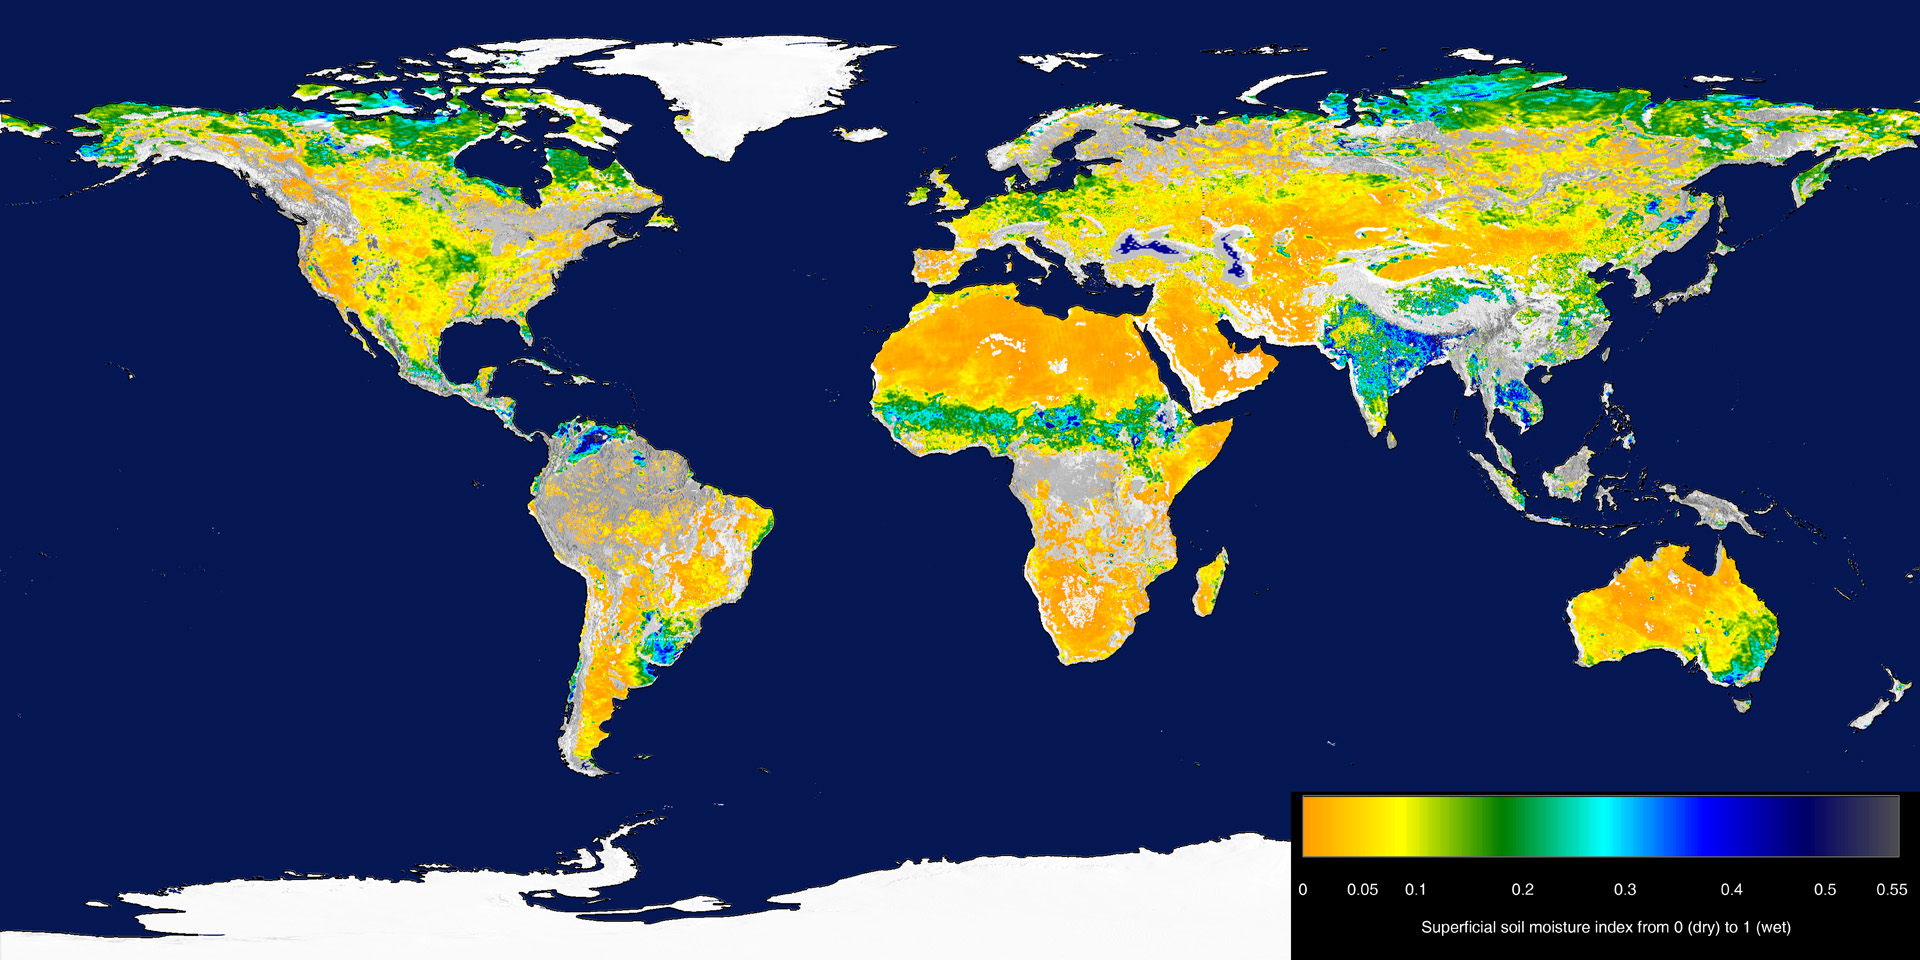
\includegraphics[width=0.75\textwidth]{fig:smos.jpg}
            \label{fig:smos}
        \end{figure}
    \end{exampleblock}
\end{frame}
%--- Next Frame ---%}

\begin{frame}{\secname : \subsecname}
    \begin{exampleblock}{Mapas de uso y cobertura - ESA/LANDCOVER}
        \begin{figure}[h!]
            \centering
            \includegraphics[width=0.75\textwidth]{fig:landcover.jpg}
            \label{fig:landcover}
        \end{figure}
    \end{exampleblock}
\end{frame}
%--- Next Frame ---%}

\begin{frame}{\secname : \subsecname}
    \begin{exampleblock}{Mapas de clorofila-a - SUOMI-NPP/VIIRS}
        \begin{figure}[h!]
            \centering
            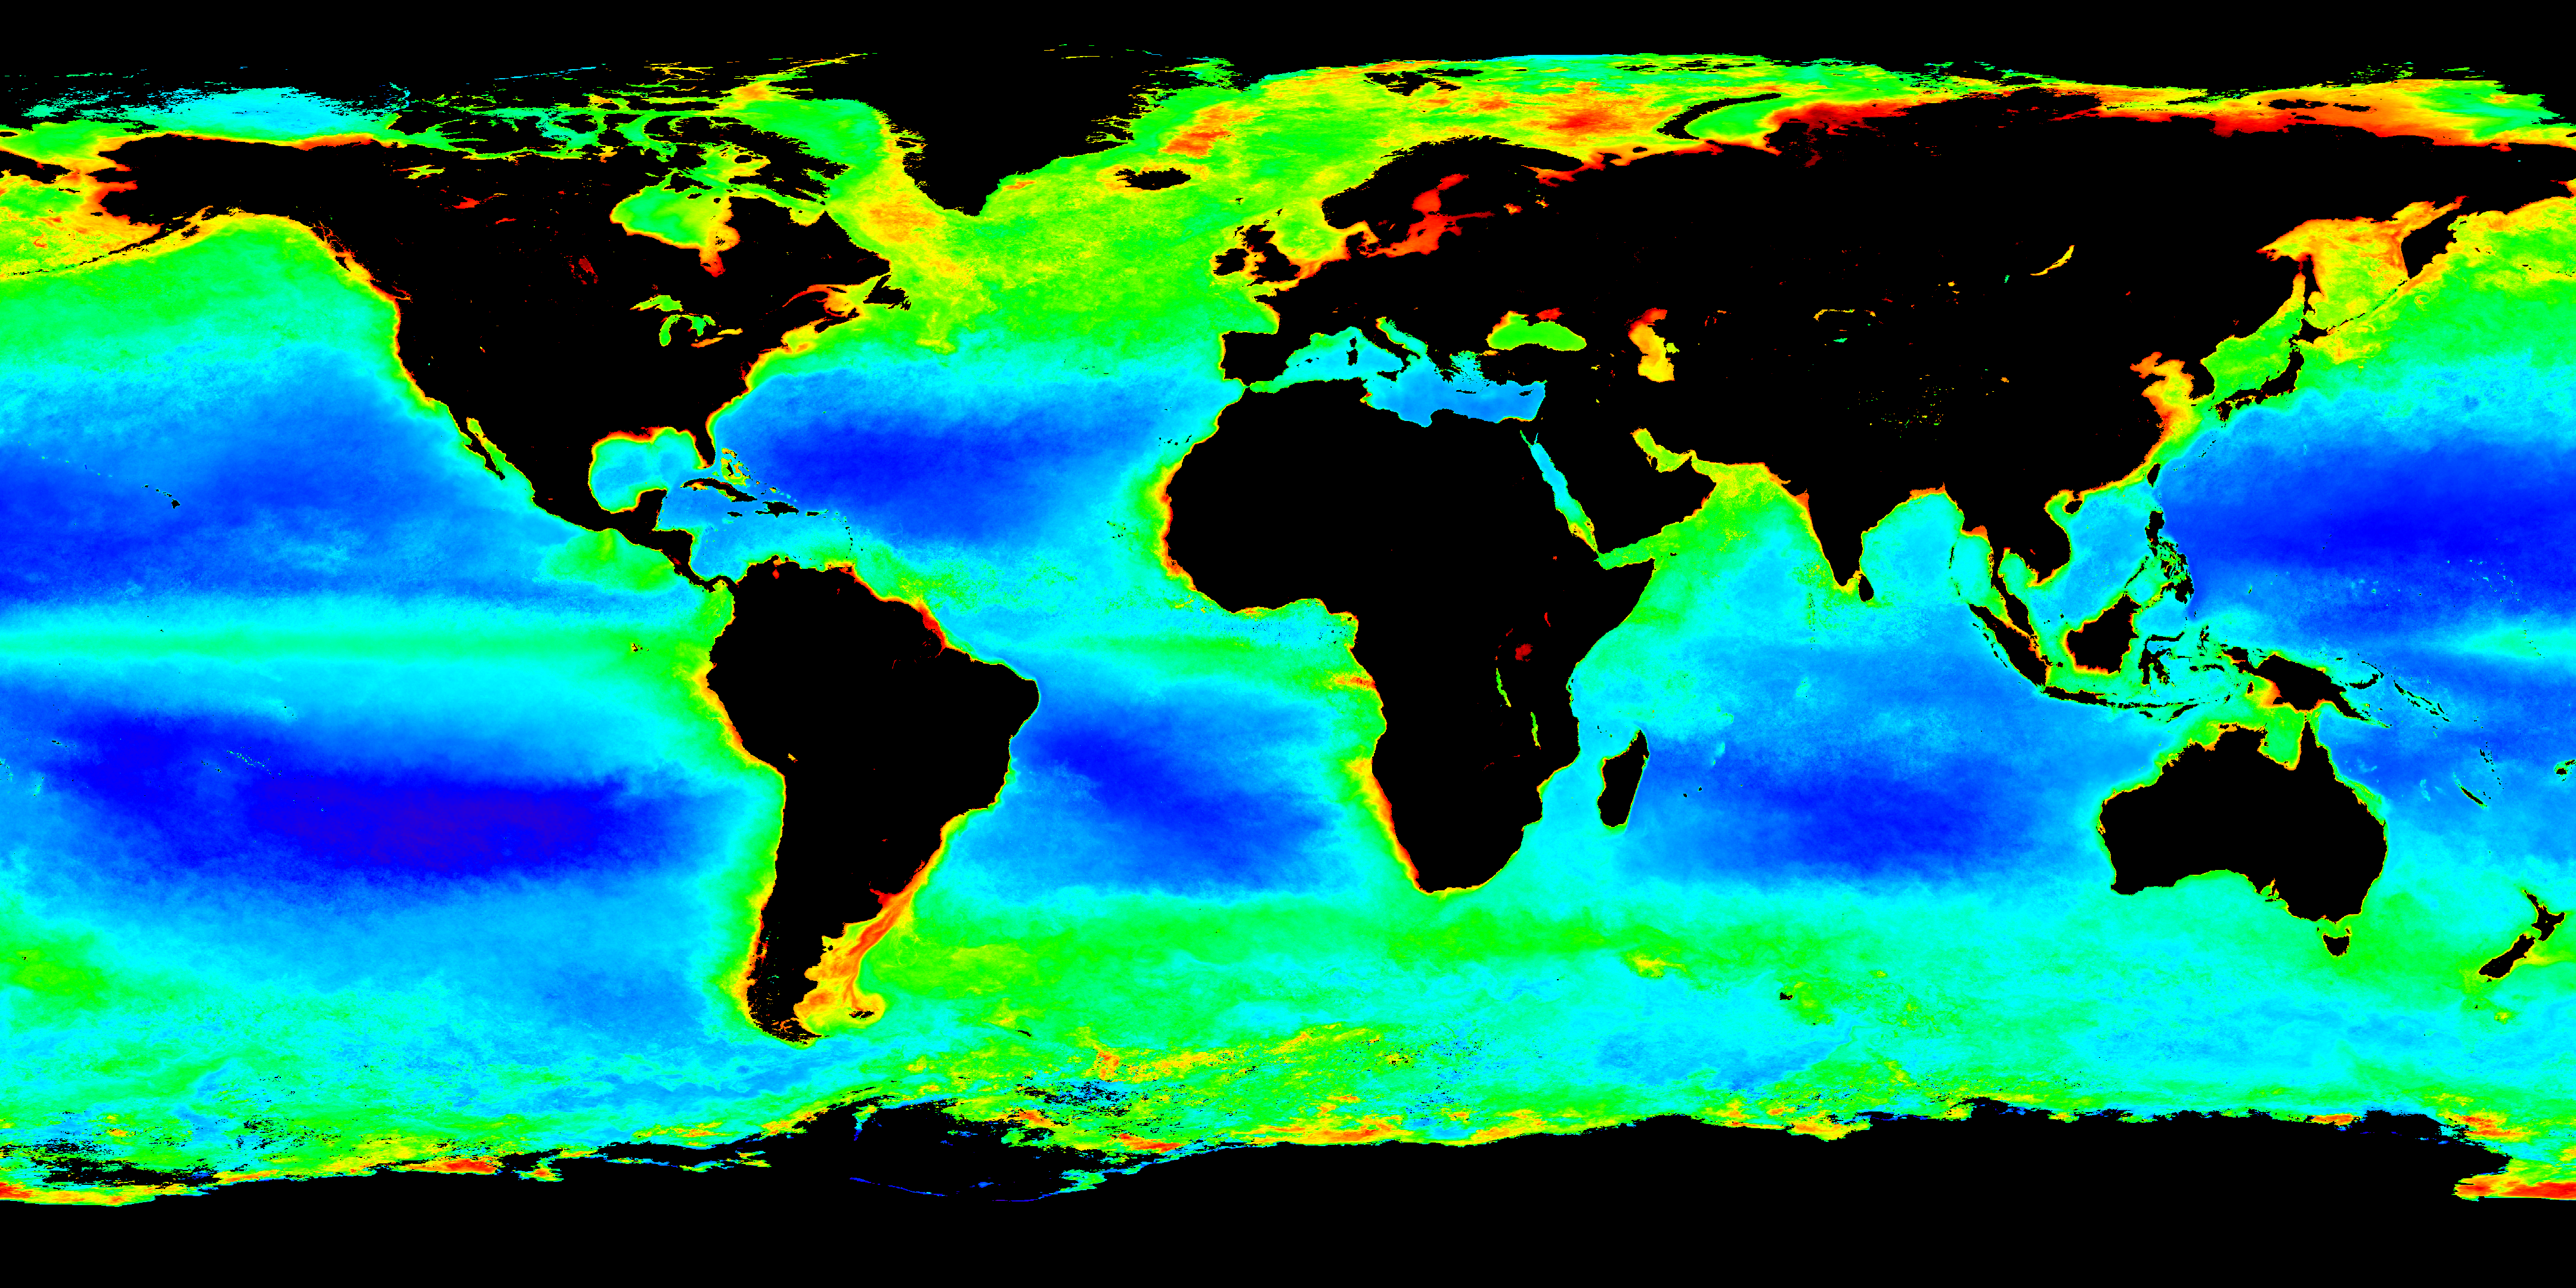
\includegraphics[width=0.75\textwidth]{fig:chl.png}
            \label{fig:chl}
        \end{figure}
    \end{exampleblock}
\end{frame}
%--- Next Frame ---%}

\section{Formas de trabajo}
\subsection{Tradicional}
\begin{frame}{\secname : \subsecname}
    \begin{itemize}[<+->]
        \item Obtención de los productos satelitales de su agencia espacial amiga.
        \item Pre-procesamiento de los productos utilizando softwares especificos de procesamiento de imagenes.
        \item Obtención de datos mediante el uso de softwares de GIS y estadísticos.
    \end{itemize}
\end{frame}
%--- Next Frame ---%

\subsection{Servicio}
\begin{frame}{\secname : \subsecname}
    \begin{itemize}[<+->]
        \item Conectarse a un sitio web que disponga de las productos deseados.
        \item Pre-procesamiento de los productos utilizando las capacidades web.
        \item Obtención de datos a partir del procesamiento y su posterior publicación.
    \end{itemize}
\end{frame}
%--- Next Frame ---%

\begin{frame}{\secname : \subsecname}
    \begin{exampleblock}{Ejemplos}
        \begin{itemize}
            \item \href{http://lv.eosda.com}{Land Viewer}
            \item \href{https://earth.google.com/web/}{Google Earth}
            \item \href{https://earthengine.google.com}{EarthEngine}
            \item \href{http://landsatexplorer.esri.com/}{LandsatExplorer}
            \item \href{http://apps.sentinel-hub.com/eo-browser/}{EO Browser}
            \item \href{https://worldview.earthdata.nasa.gov/}{Nasa WorldView}
            \item \href{http://maps.elie.ucl.ac.be/CCI/viewer/index.php}{Land Cover Maps}
            \item Y creciendo...
        \end{itemize}
    \end{exampleblock}
\end{frame}
%--- Next Frame ---%

\subsection{Actividad}

\begin{frame}{\secname : \subsecname}
    \begin{alertblock}{Land Viewer}
        Medición de distancias, áreas y posiciones en el Land Viewer de EOSDA.
    \end{alertblock}
\end{frame}
%--- Next Frame ---%


\section{Resolución espacial y temporal}
\subsection{Resolución espacial}
\begin{frame}{\secname : \subsecname}
    \begin{block}{Definición}
        Es la capacidad del sensor de distinguir objetos en el terreno.
    \end{block}
\end{frame}
%--- Next Frame ---%

\begin{frame}{\secname : \subsecname}
    \begin{figure}[h!]
        \centering
        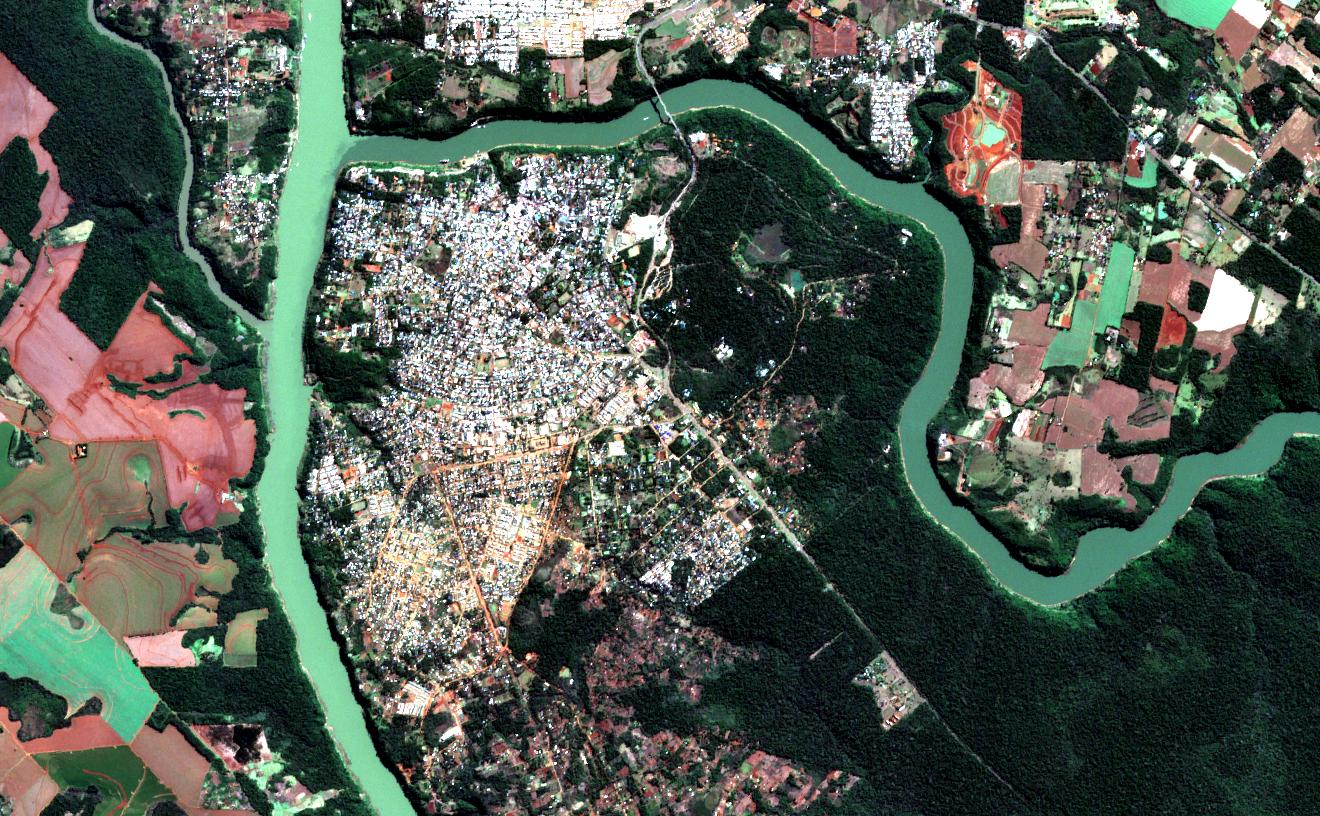
\includegraphics[width=0.7\textwidth]{fig:10m.jpg}
        \caption{Imagen con resolución espacial de 10m.}
    \end{figure}
\end{frame}
%--- Next Frame ---%

\begin{frame}{\secname : \subsecname}
    \begin{figure}[h!]
        \centering
        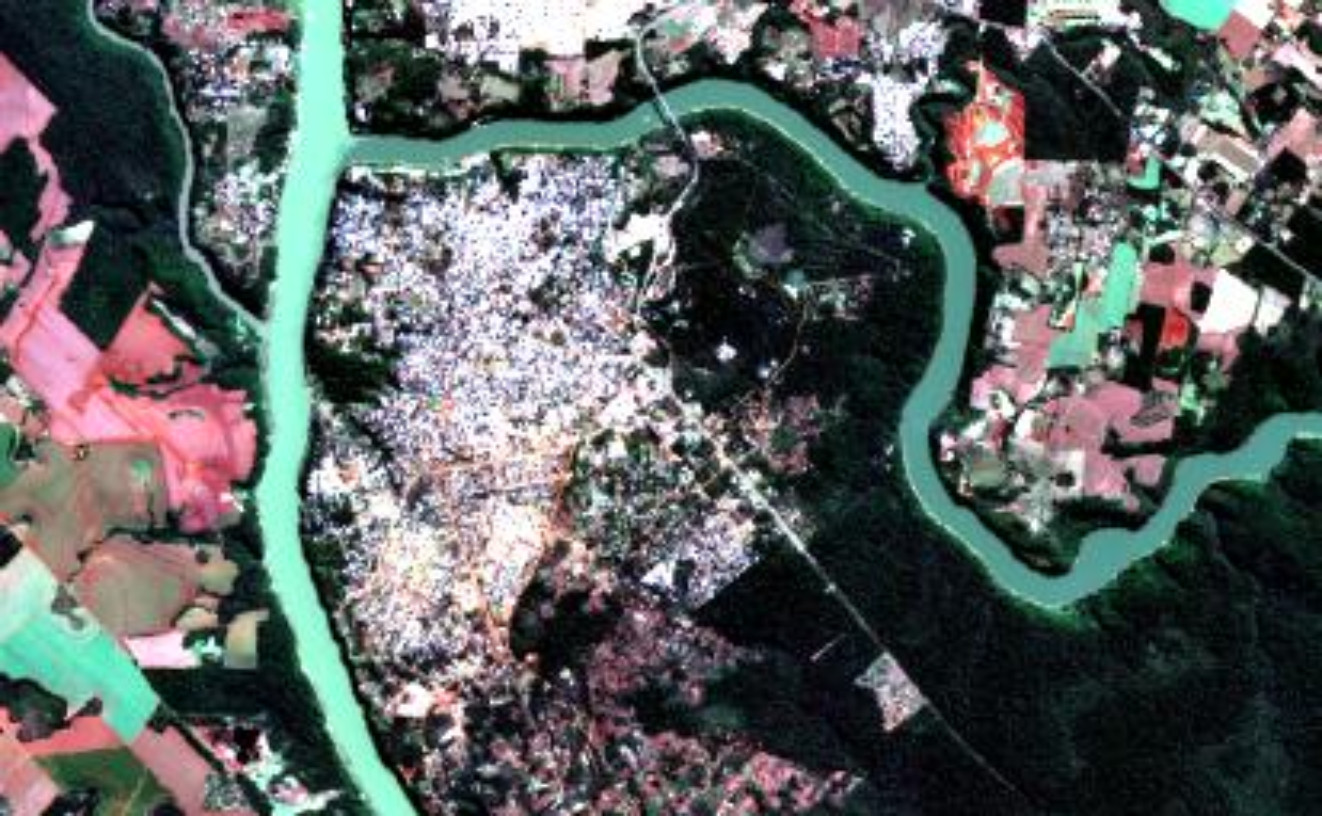
\includegraphics[width=0.7\textwidth]{fig:30m.jpg}
        \caption{Imagen con resolución espacial de 30m.}
    \end{figure}
\end{frame}
%--- Next Frame ---%

\begin{frame}{\secname : \subsecname}
    \begin{figure}[h!]
        \centering
        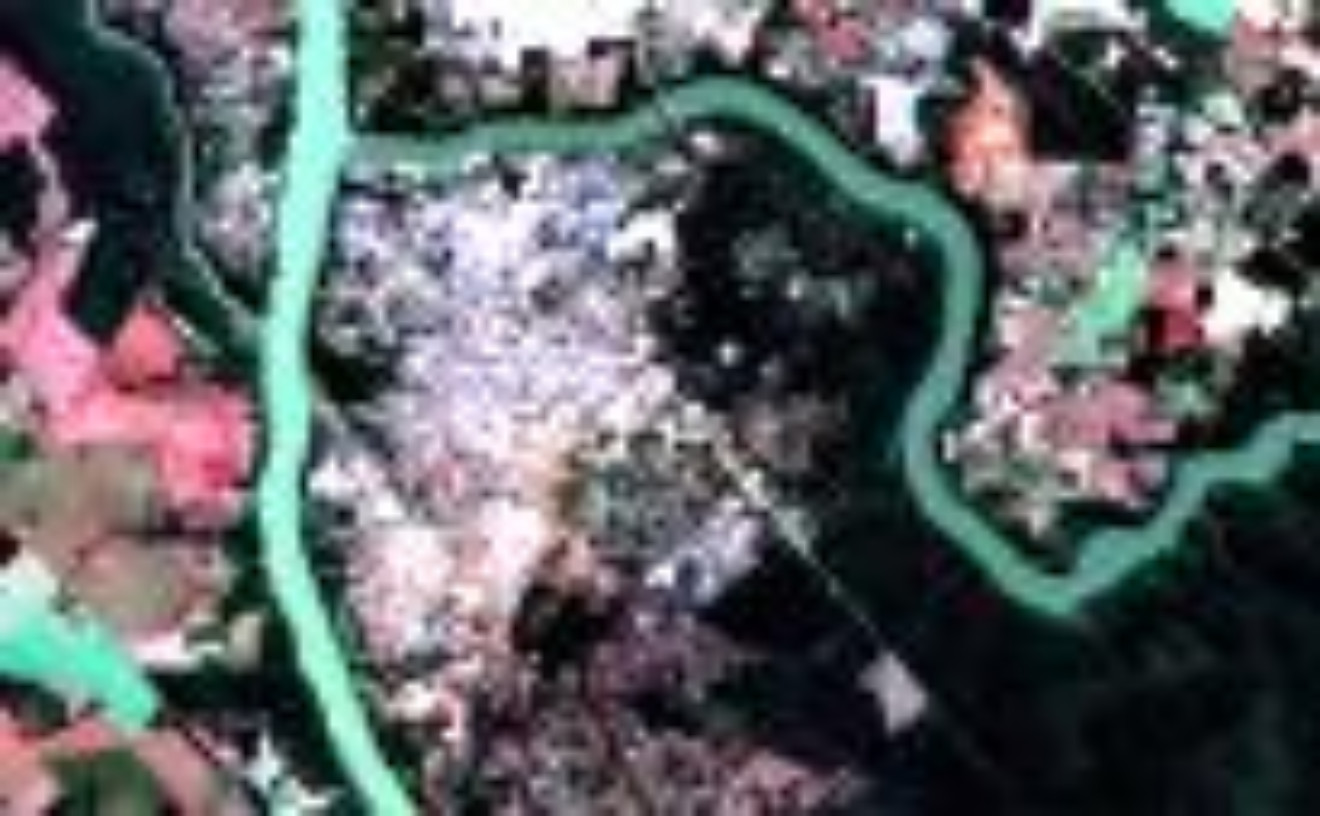
\includegraphics[width=0.7\textwidth]{fig:90m.jpg}
        \caption{Imagen con resolución espacial de 90m.}
    \end{figure}
\end{frame}
%--- Next Frame ---%

\begin{frame}{\secname : \subsecname}
    \begin{figure}[h!]
        \centering
        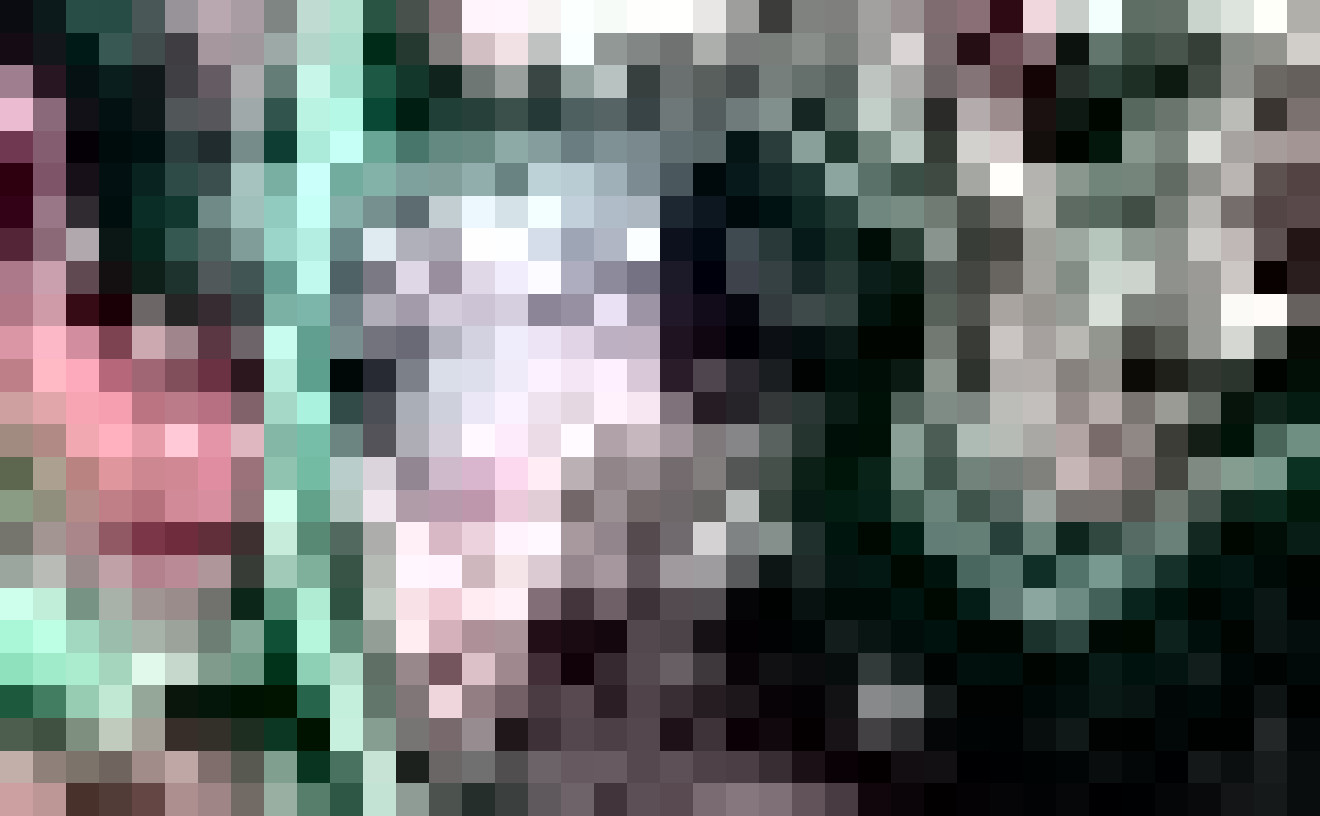
\includegraphics[width=0.7\textwidth]{fig:300m.jpg}
        \caption{Imagen con resolución espacial de 300m.}
    \end{figure}
\end{frame}
%--- Next Frame ---%

\begin{frame}{\secname : \subsecname}
    \begin{figure}[h!]
        \centering
        
\includegraphics[width=0.7\textwidth]{fig:1000m.jpg}
        \caption{Imagen con resolución espacial de 1000m.}
    \end{figure}
\end{frame}
%--- Next Frame ---%

\subsection{Resolución temporal}

\begin{frame}{\secname : \subsecname}
    \begin{block}{Definición}
        Es la capacidad del sensor de distinguir cambios en el tiempo.
    \end{block}
\end{frame}
%--- Next Frame ---%

\begin{frame}{\secname : \subsecname}
    \begin{figure}[h!]
        \centering
        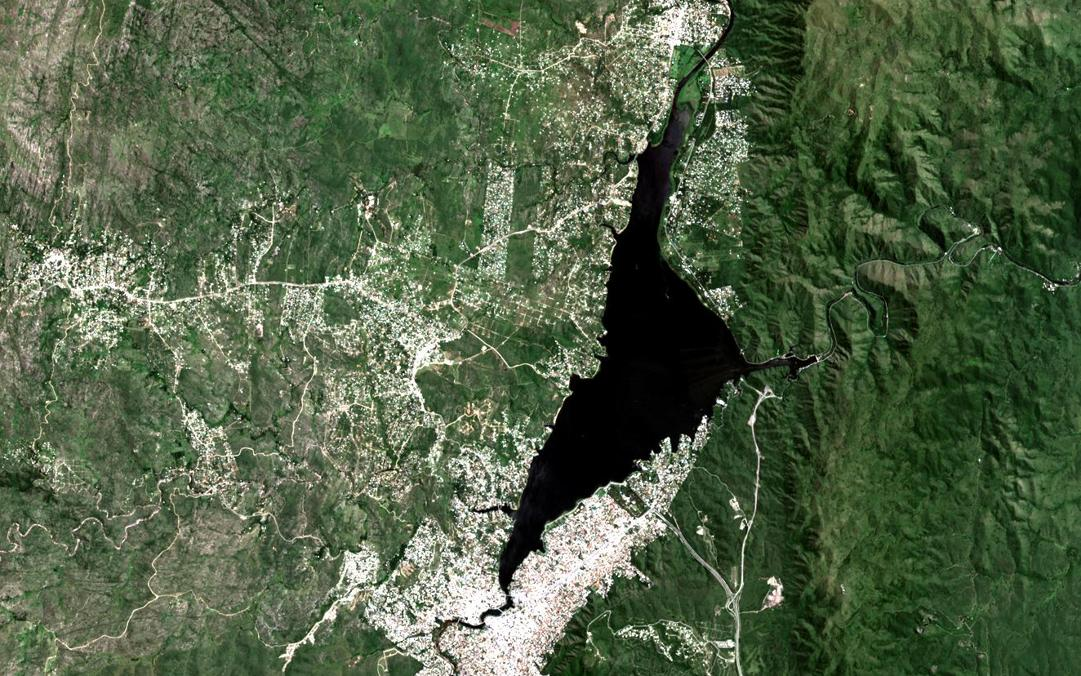
\includegraphics[width=0.6\textwidth]{fig:lake-beg.jpeg}
        \caption{Evolución temporal del contenido de clorofila en superficie en el lago San Roque. Imagen del 12 de febrero de 2017.}
        \label{fig:lake-beg}
    \end{figure}
\end{frame}
%--- Next Frame ---%

\begin{frame}{\secname : \subsecname}
    \begin{figure}[h!]
        \centering
        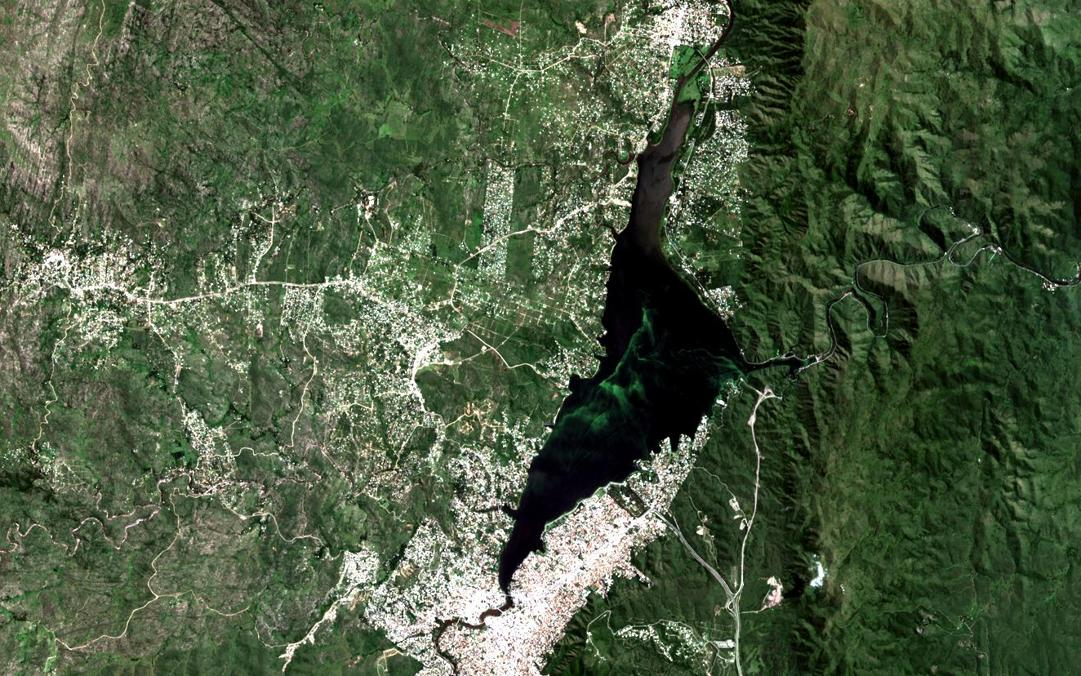
\includegraphics[width=0.6\textwidth]{fig:lake-end.jpeg}
        \caption{Evolución temporal del contenido de clorofila en superficie en el lago San Roque. Imagen del 22 de febrero de 2017.}
        \label{fig:lake-end}
    \end{figure}
\end{frame}
%--- Next Frame ---%

\begin{frame}{\secname : \subsecname}
    \begin{figure}[h!]
        \centering
        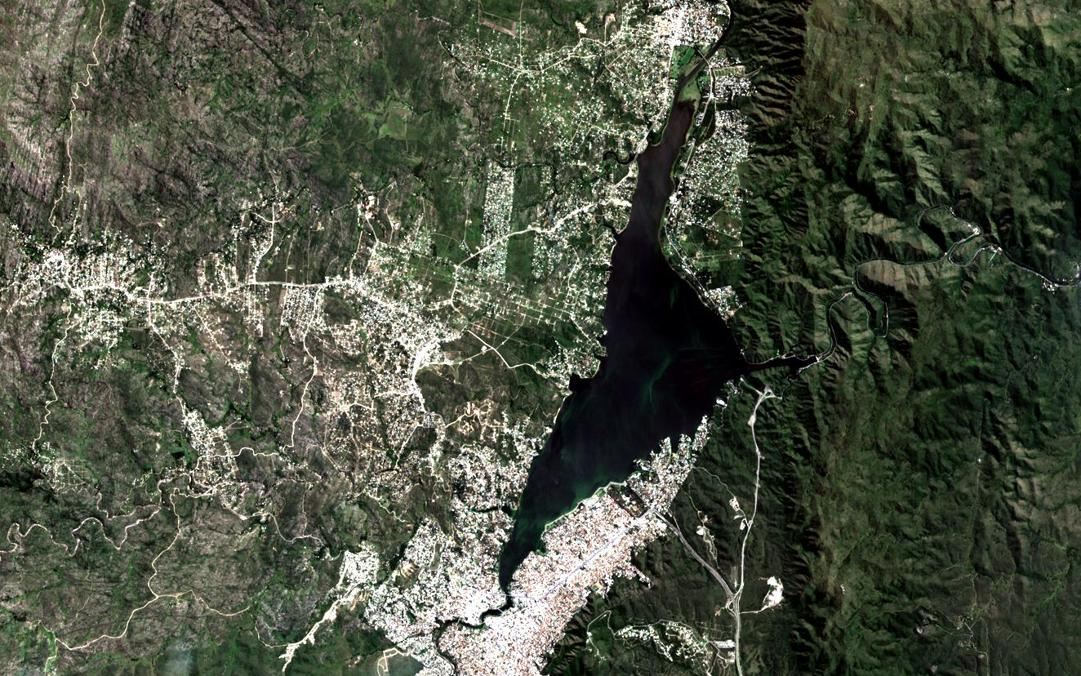
\includegraphics[width=0.6\textwidth]{fig:lake-aft.jpeg}
        \caption{Evolución temporal del contenido de clorofila en superficie en el lago San Roque. Imagen del 14 de marzo de 2017. (\href{https://goo.gl/M5595z}{https://goo.gl/M5595z}).}
        \label{fig:lake-aft}
    \end{figure}
\end{frame}
%--- Next Frame ---%

\begin{frame}{\secname : \subsecname}
    \begin{figure}[h!]
    \centering
    \movie[width = 0.6 \textwidth,loop]{\centering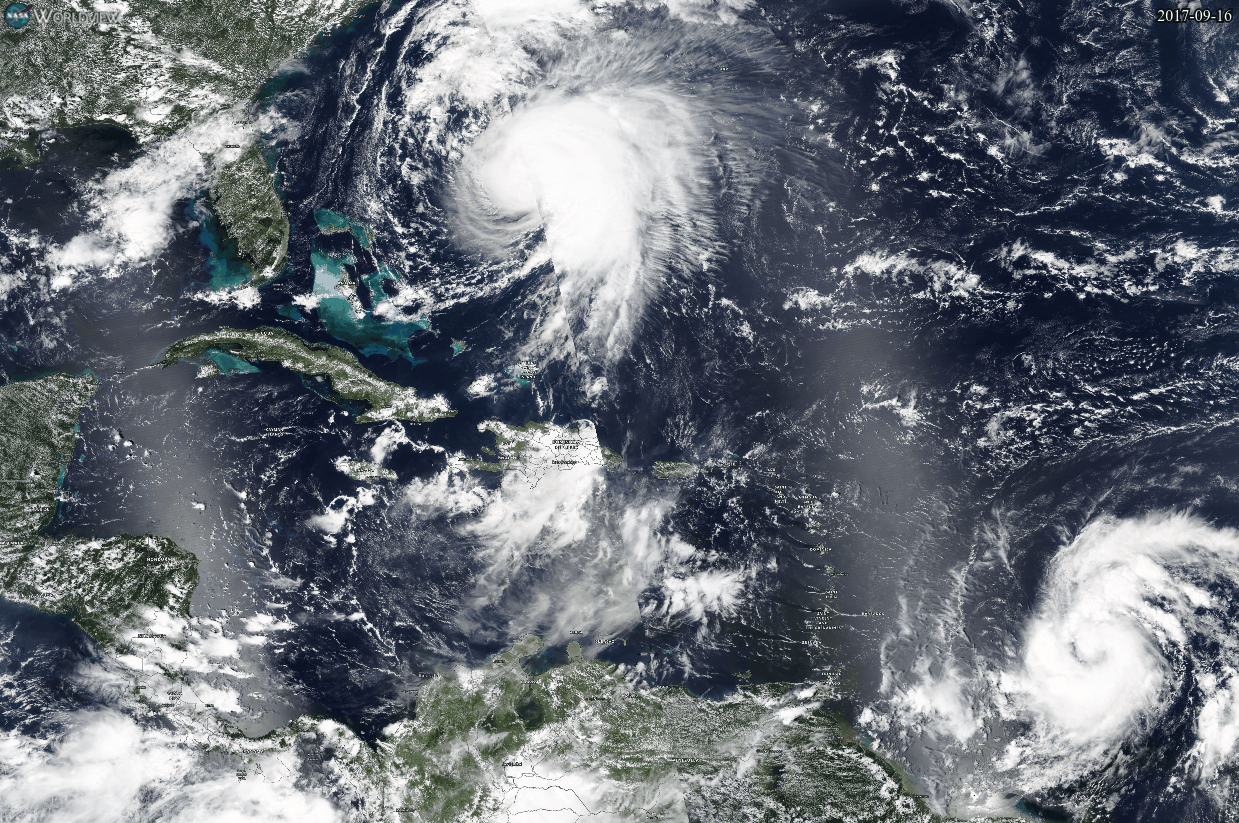
\includegraphics[width=0.6\textwidth]{Pic.png}}{./figs/1.mp4}
    \caption{Evolución del huracan Maria en el mes de septiembre. (\href{https://goo.gl/M5595z}{https://goo.gl/M5595z}).}
    \end{figure}
\end{frame}
%--- Next Frame ---%


\subsection{Aplicaciones}

\begin{frame}{\secname : \subsecname}
    \begin{figure}[h!]
        \centering
        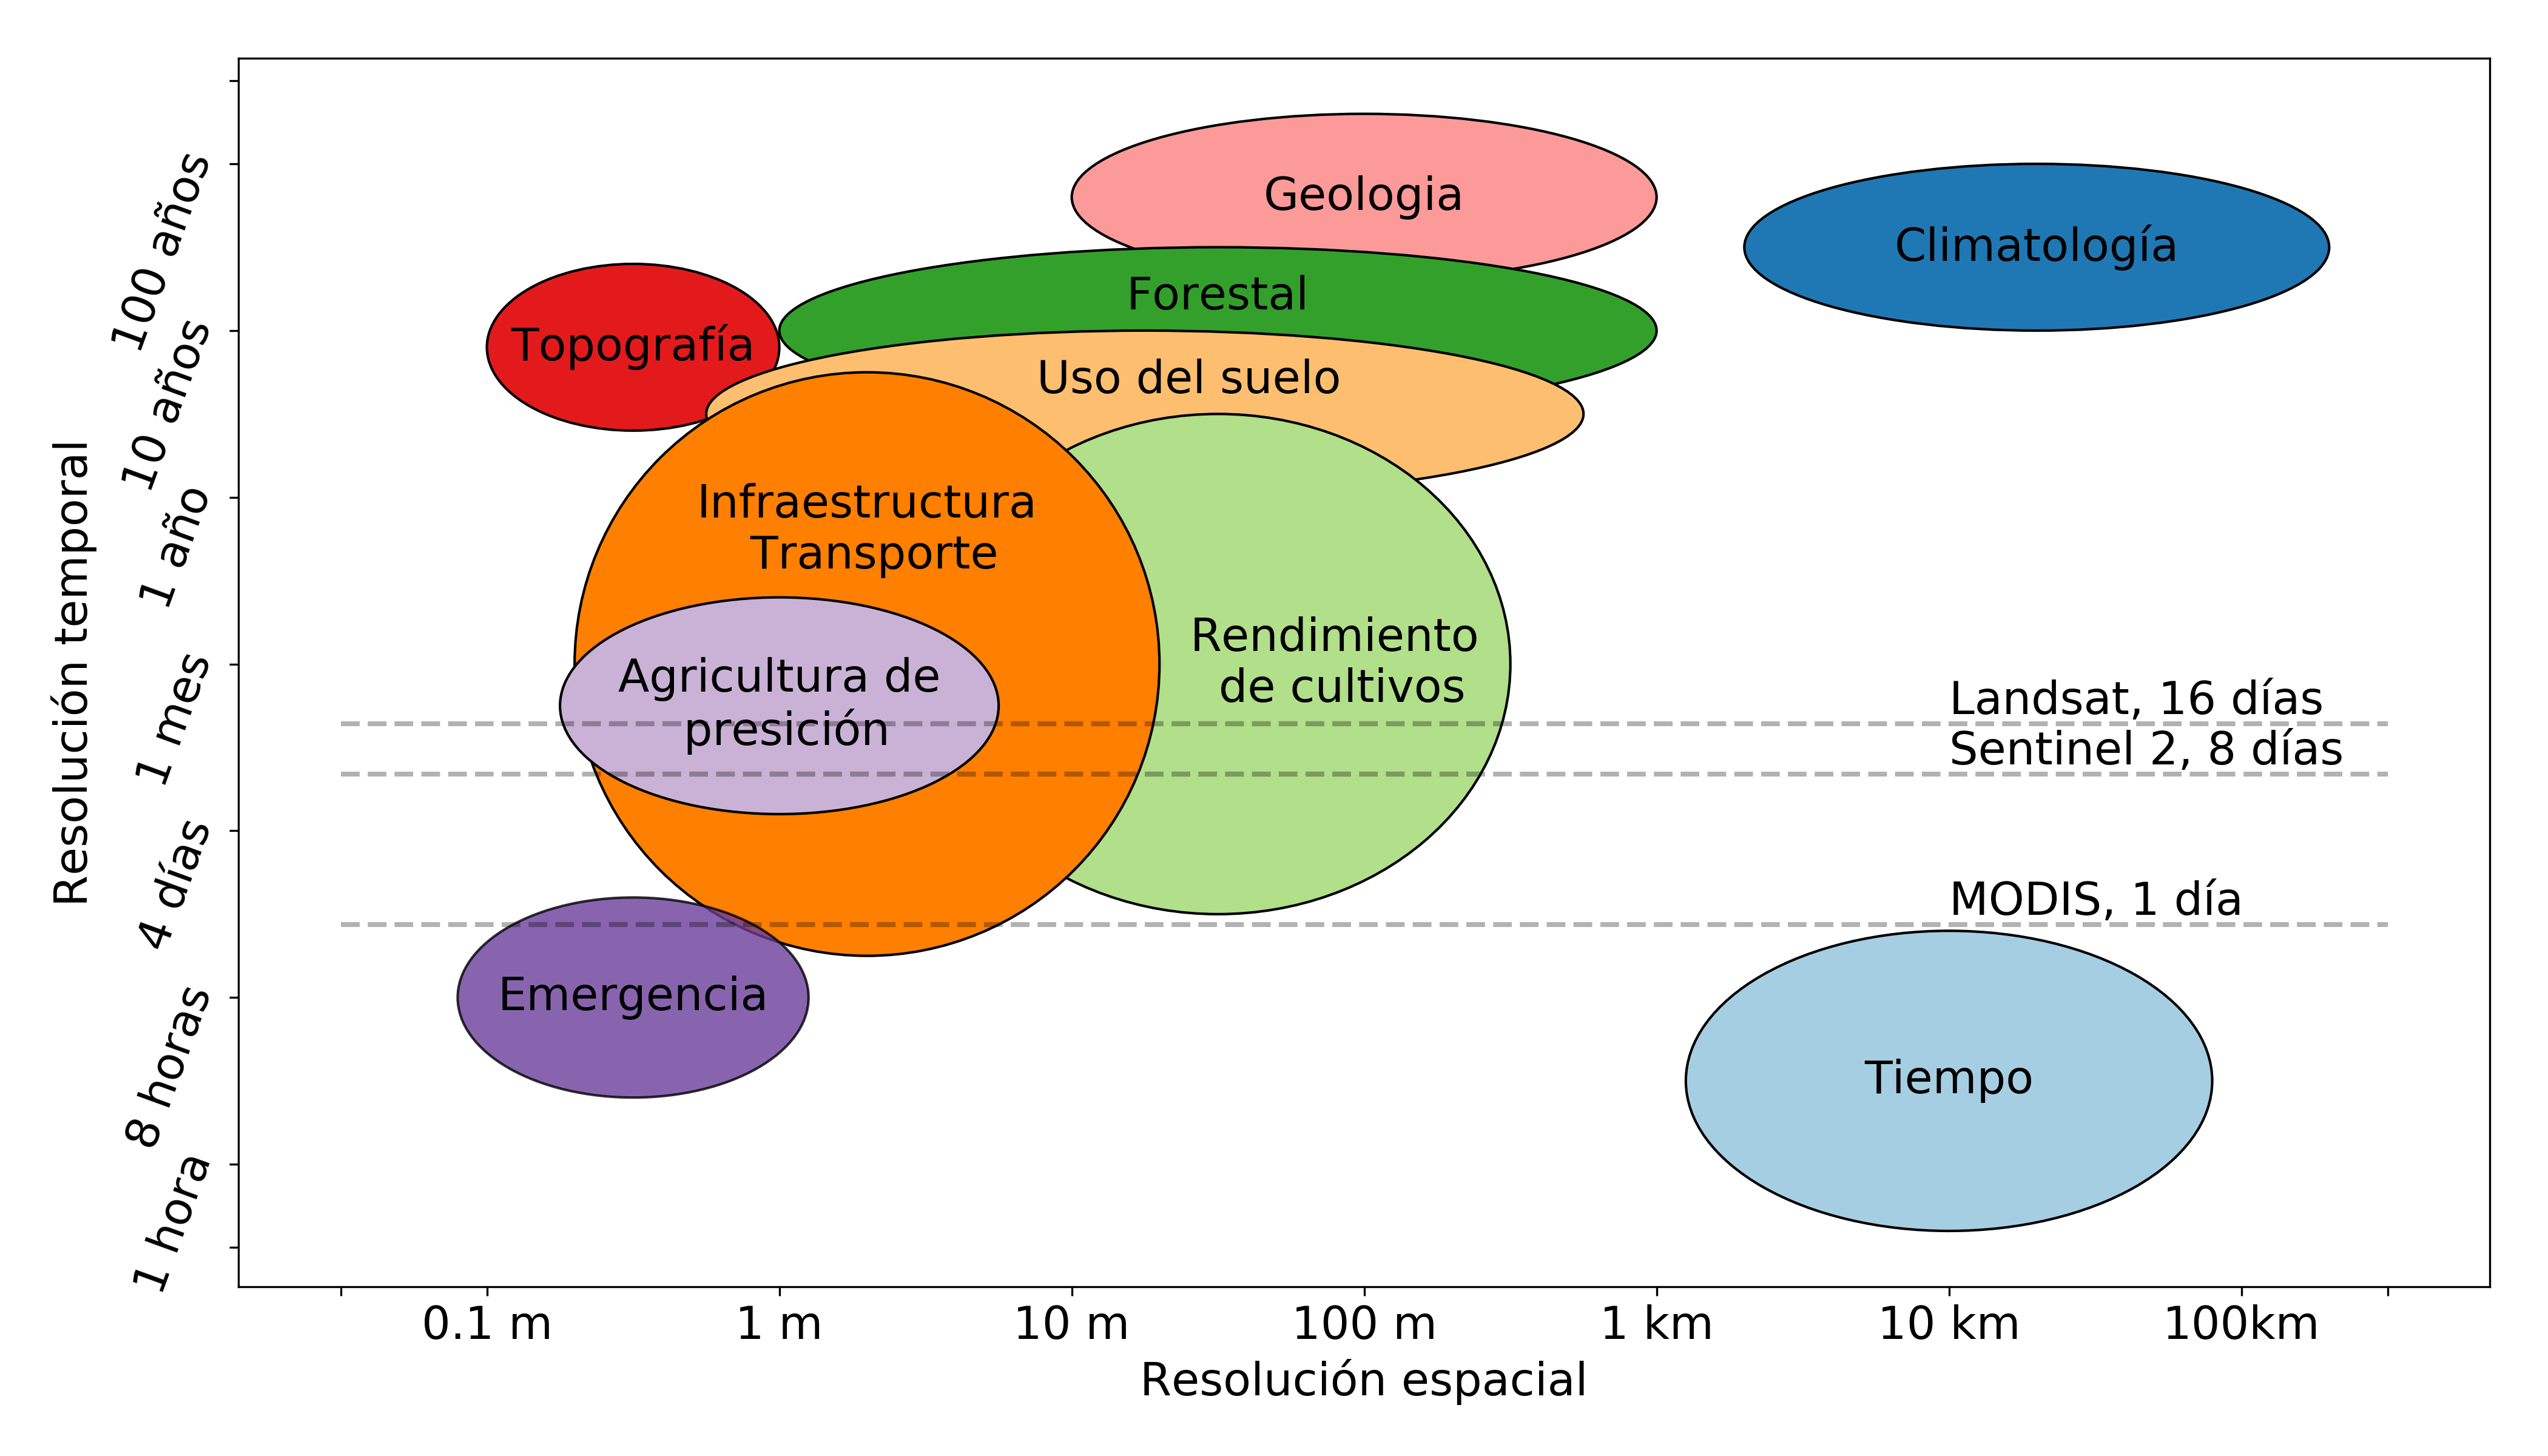
\includegraphics[width=0.7\textwidth]{fig:evst.png}
        \caption{Comparación de distintos usos de productos satelitales y las resoluciones espaciales y temporales necesarias.}
        \label{fig:evst}
    \end{figure}
\end{frame}
%--- Next Frame ---%

\subsection{Actividad}

\begin{frame}{\secname : \subsecname}
    \begin{alertblock}{Resolución espacial y temporal}
        Comparación de imágenes con distintas resoluciones espaciles y temporales.
    \end{alertblock}
\end{frame}
%--- Next Frame ---%


\section{Combinaciones espectrales}
\subsection{Luz visible}

\begin{frame}{\secname : \subsecname}
    \begin{figure}[h!]
        \centering
        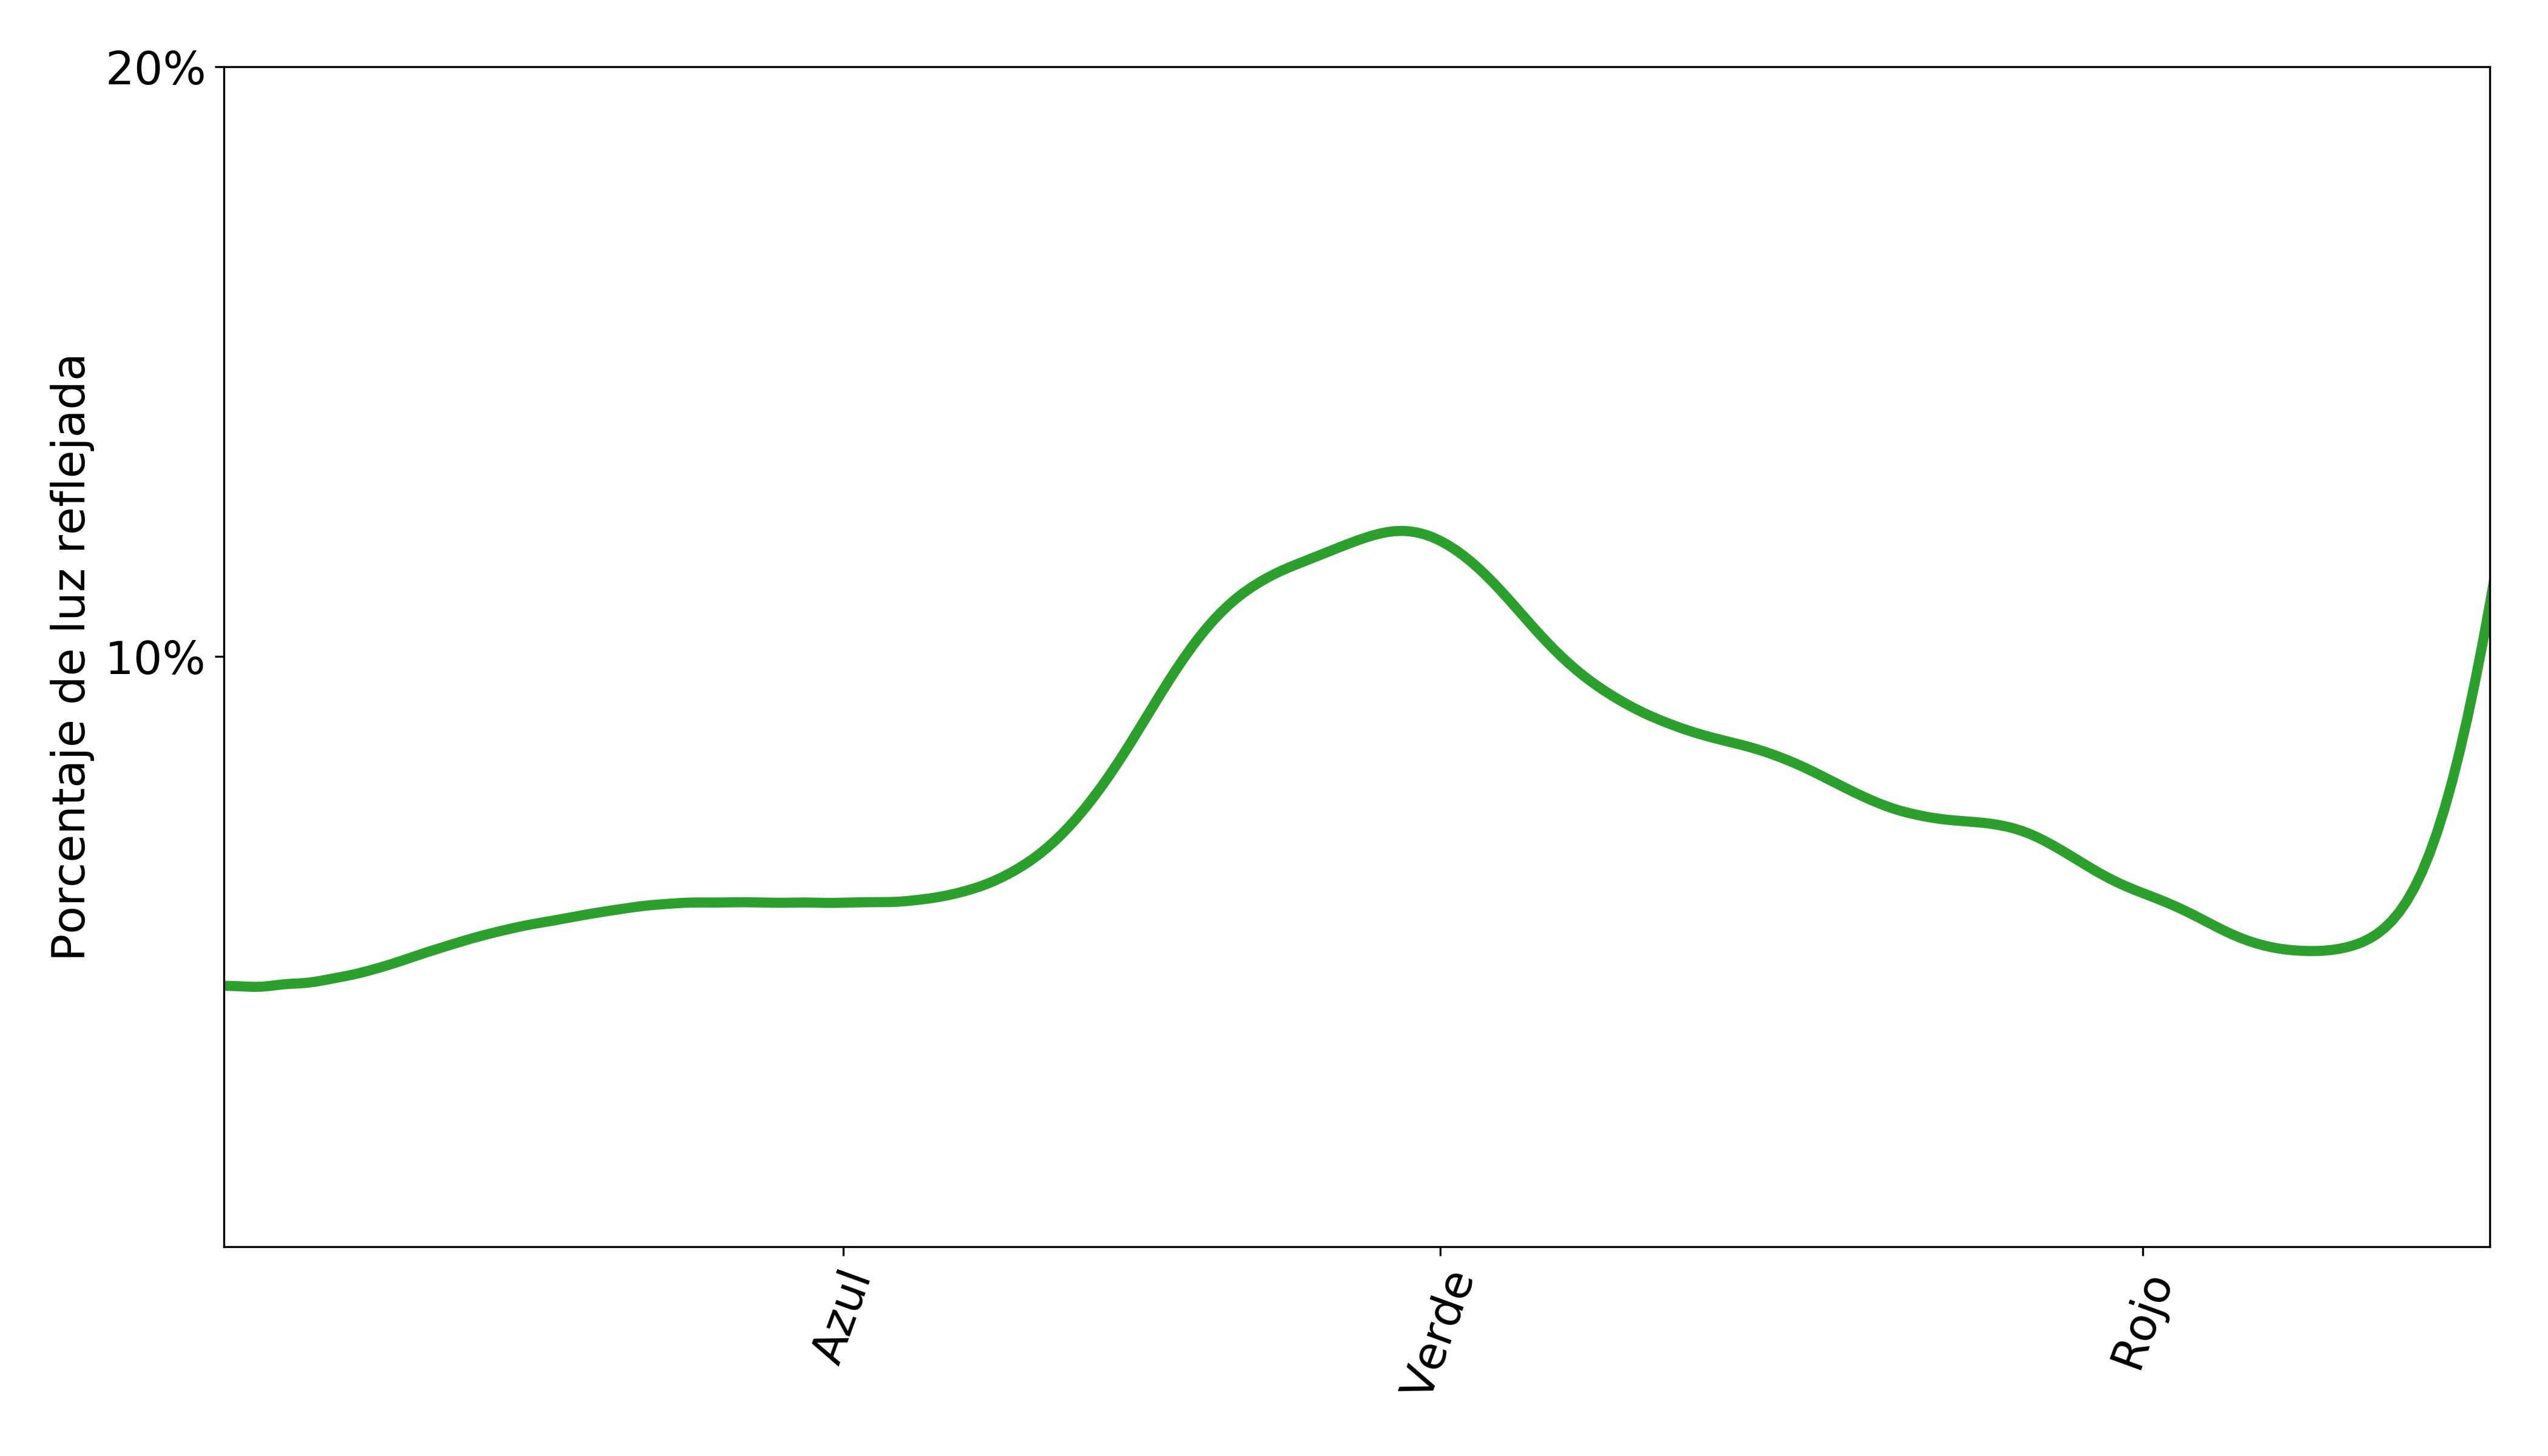
\includegraphics[width=0.8\textwidth]{fig:v.png}
        \caption{Firma espectral de la vegetación en el espectro visible.}
        \label{fig:v}
    \end{figure}
\end{frame}
%--- Next Frame ---%

\begin{frame}{\secname : \subsecname}
    \begin{figure}[h!]
        \centering
        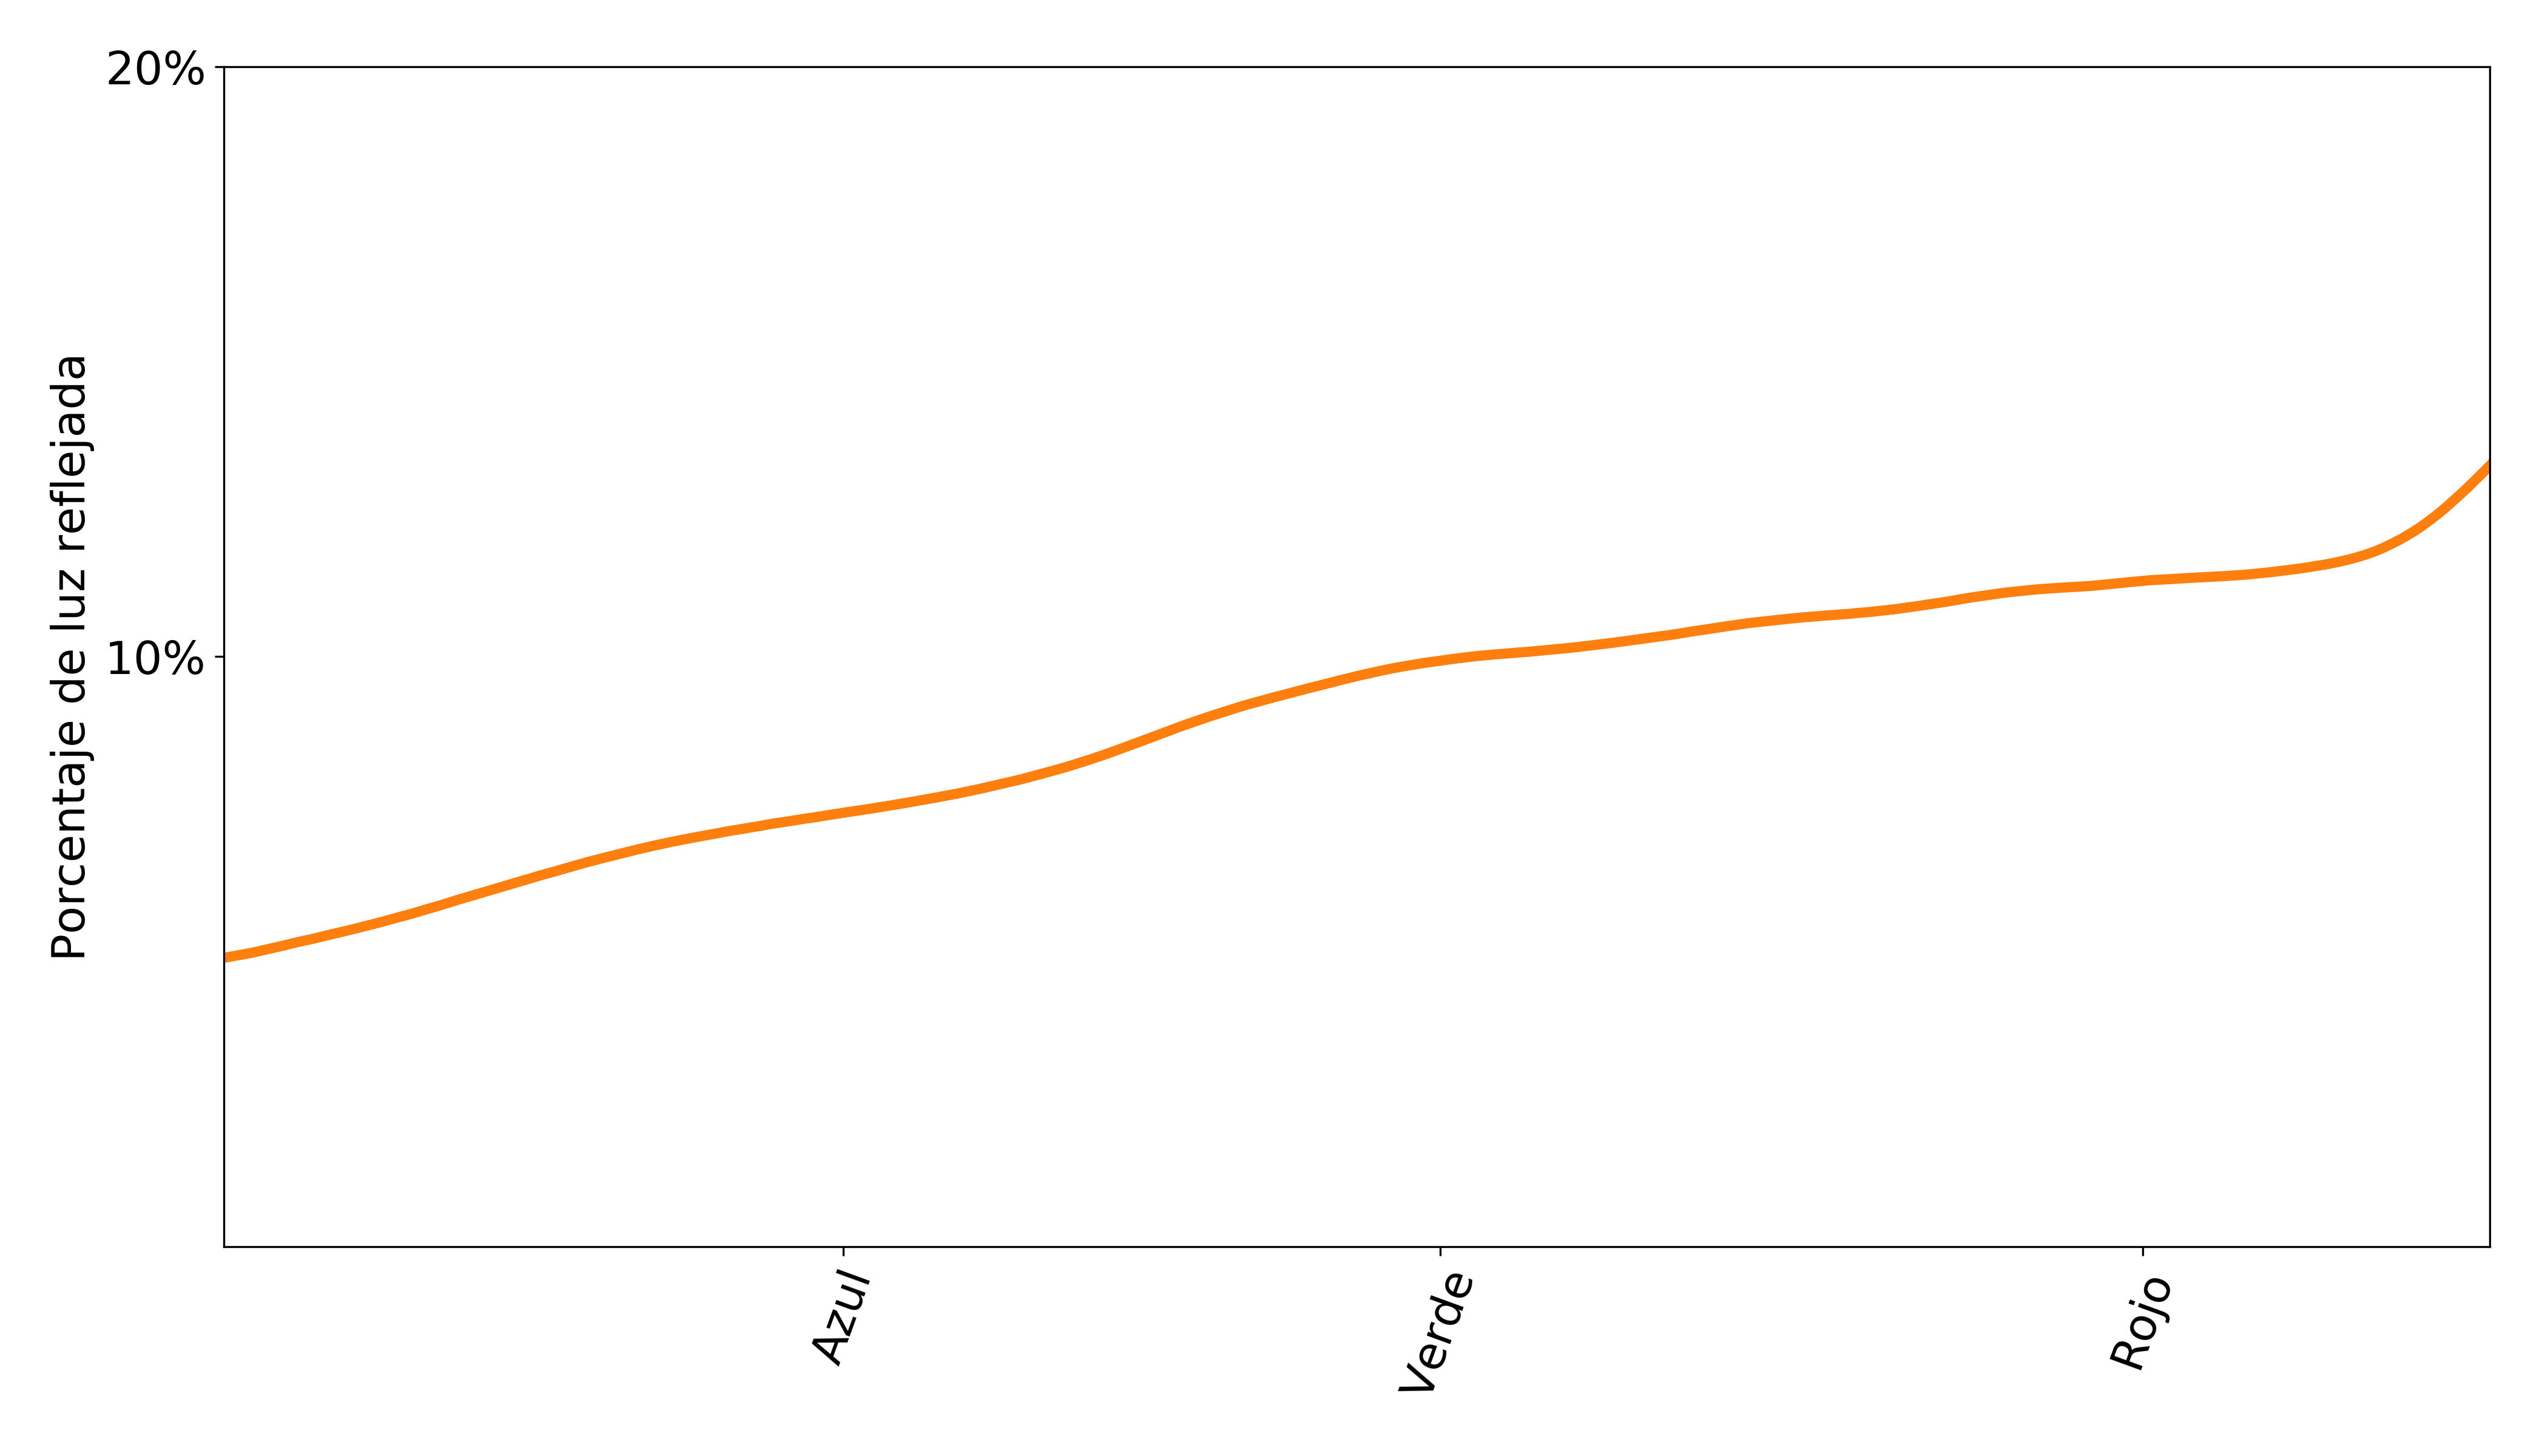
\includegraphics[width=0.8\textwidth]{fig:s.png}
        \caption{Firma espectral del suelo en el espectro visible.}
        \label{fig:s}
    \end{figure}
\end{frame}
%--- Next Frame ---%

\begin{frame}{\secname : \subsecname}
    \begin{figure}[h!]
        \centering
        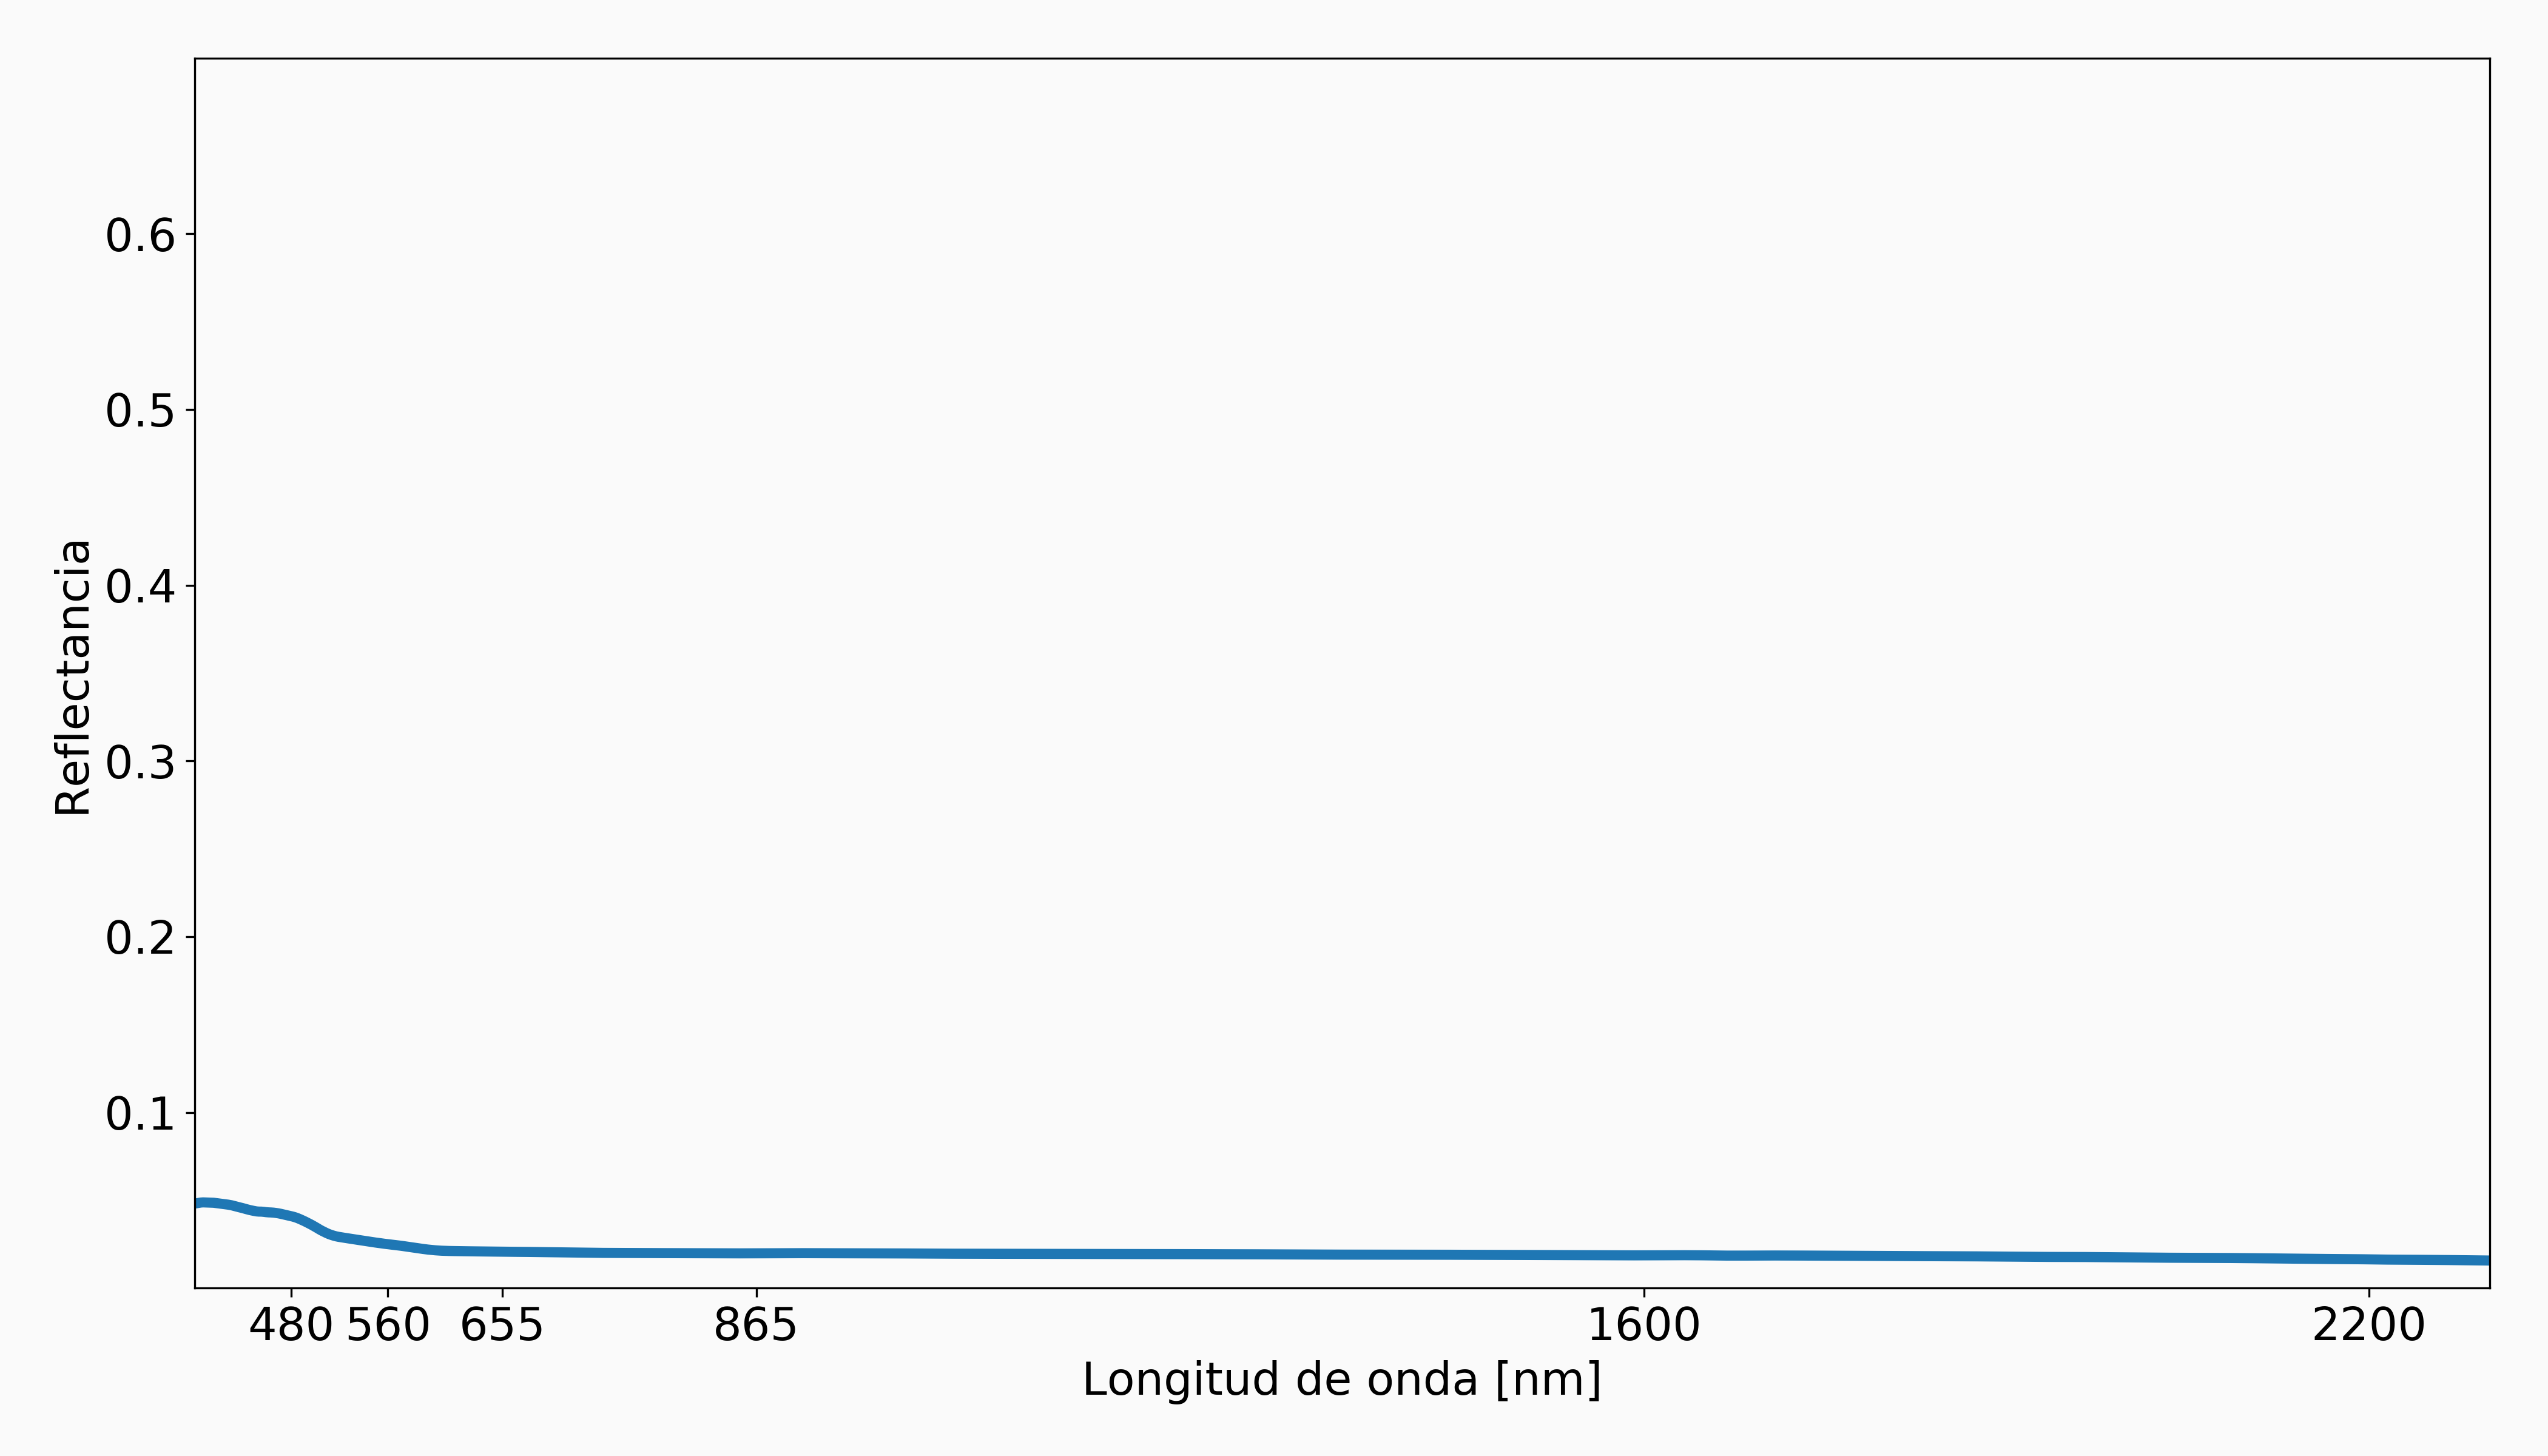
\includegraphics[width=0.8\textwidth]{fig:a.png}
        \caption{Firma espectral del agua en el espectro visible.}
        \label{fig:a}
    \end{figure}
\end{frame}
%--- Next Frame ---%

\subsection{Luz no visible}

\begin{frame}{\secname : \subsecname}
    \begin{figure}[h!]
        \centering
        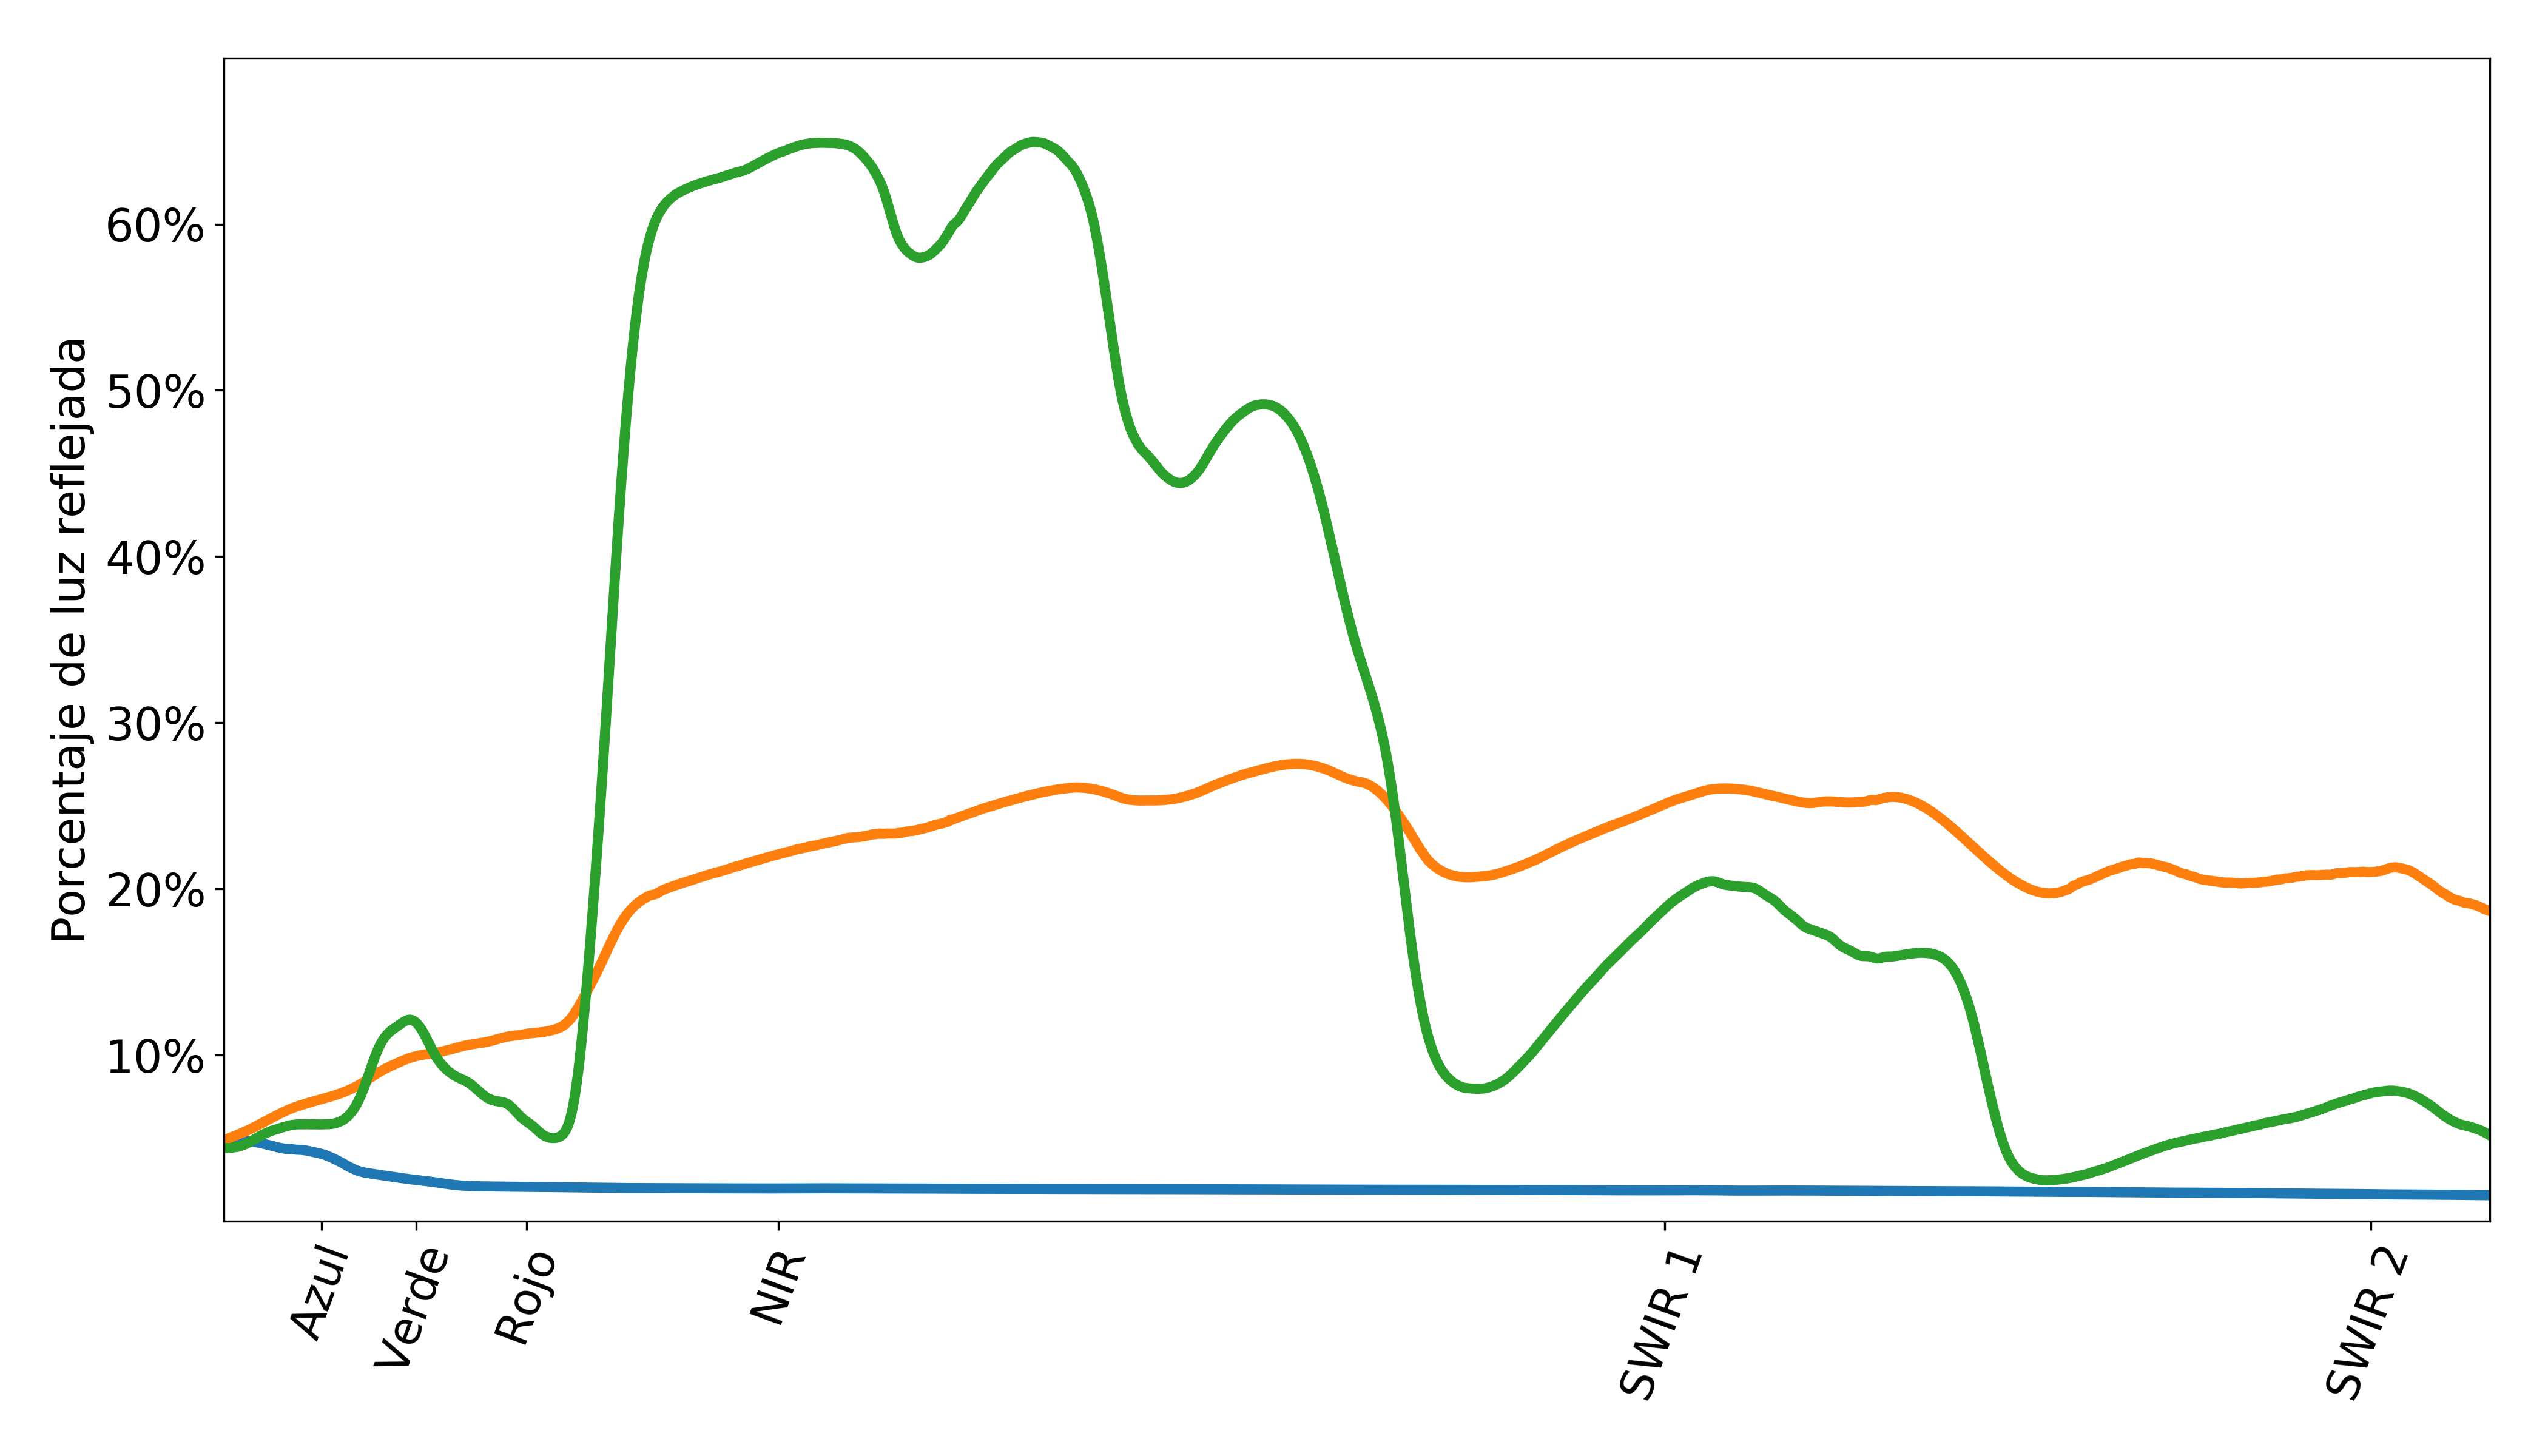
\includegraphics[width=0.8\textwidth]{fig:spec.png}
        \caption{Firmas espectrales de distintass coberturas en otras zonas del espectro.}
        \label{fig:spec}
    \end{figure}
\end{frame}
%--- Next Frame ---%

\subsection{Combinaciones típicas}

\begin{frame}{\secname : \subsecname}
    \begin{figure}[h!]
        \centering
        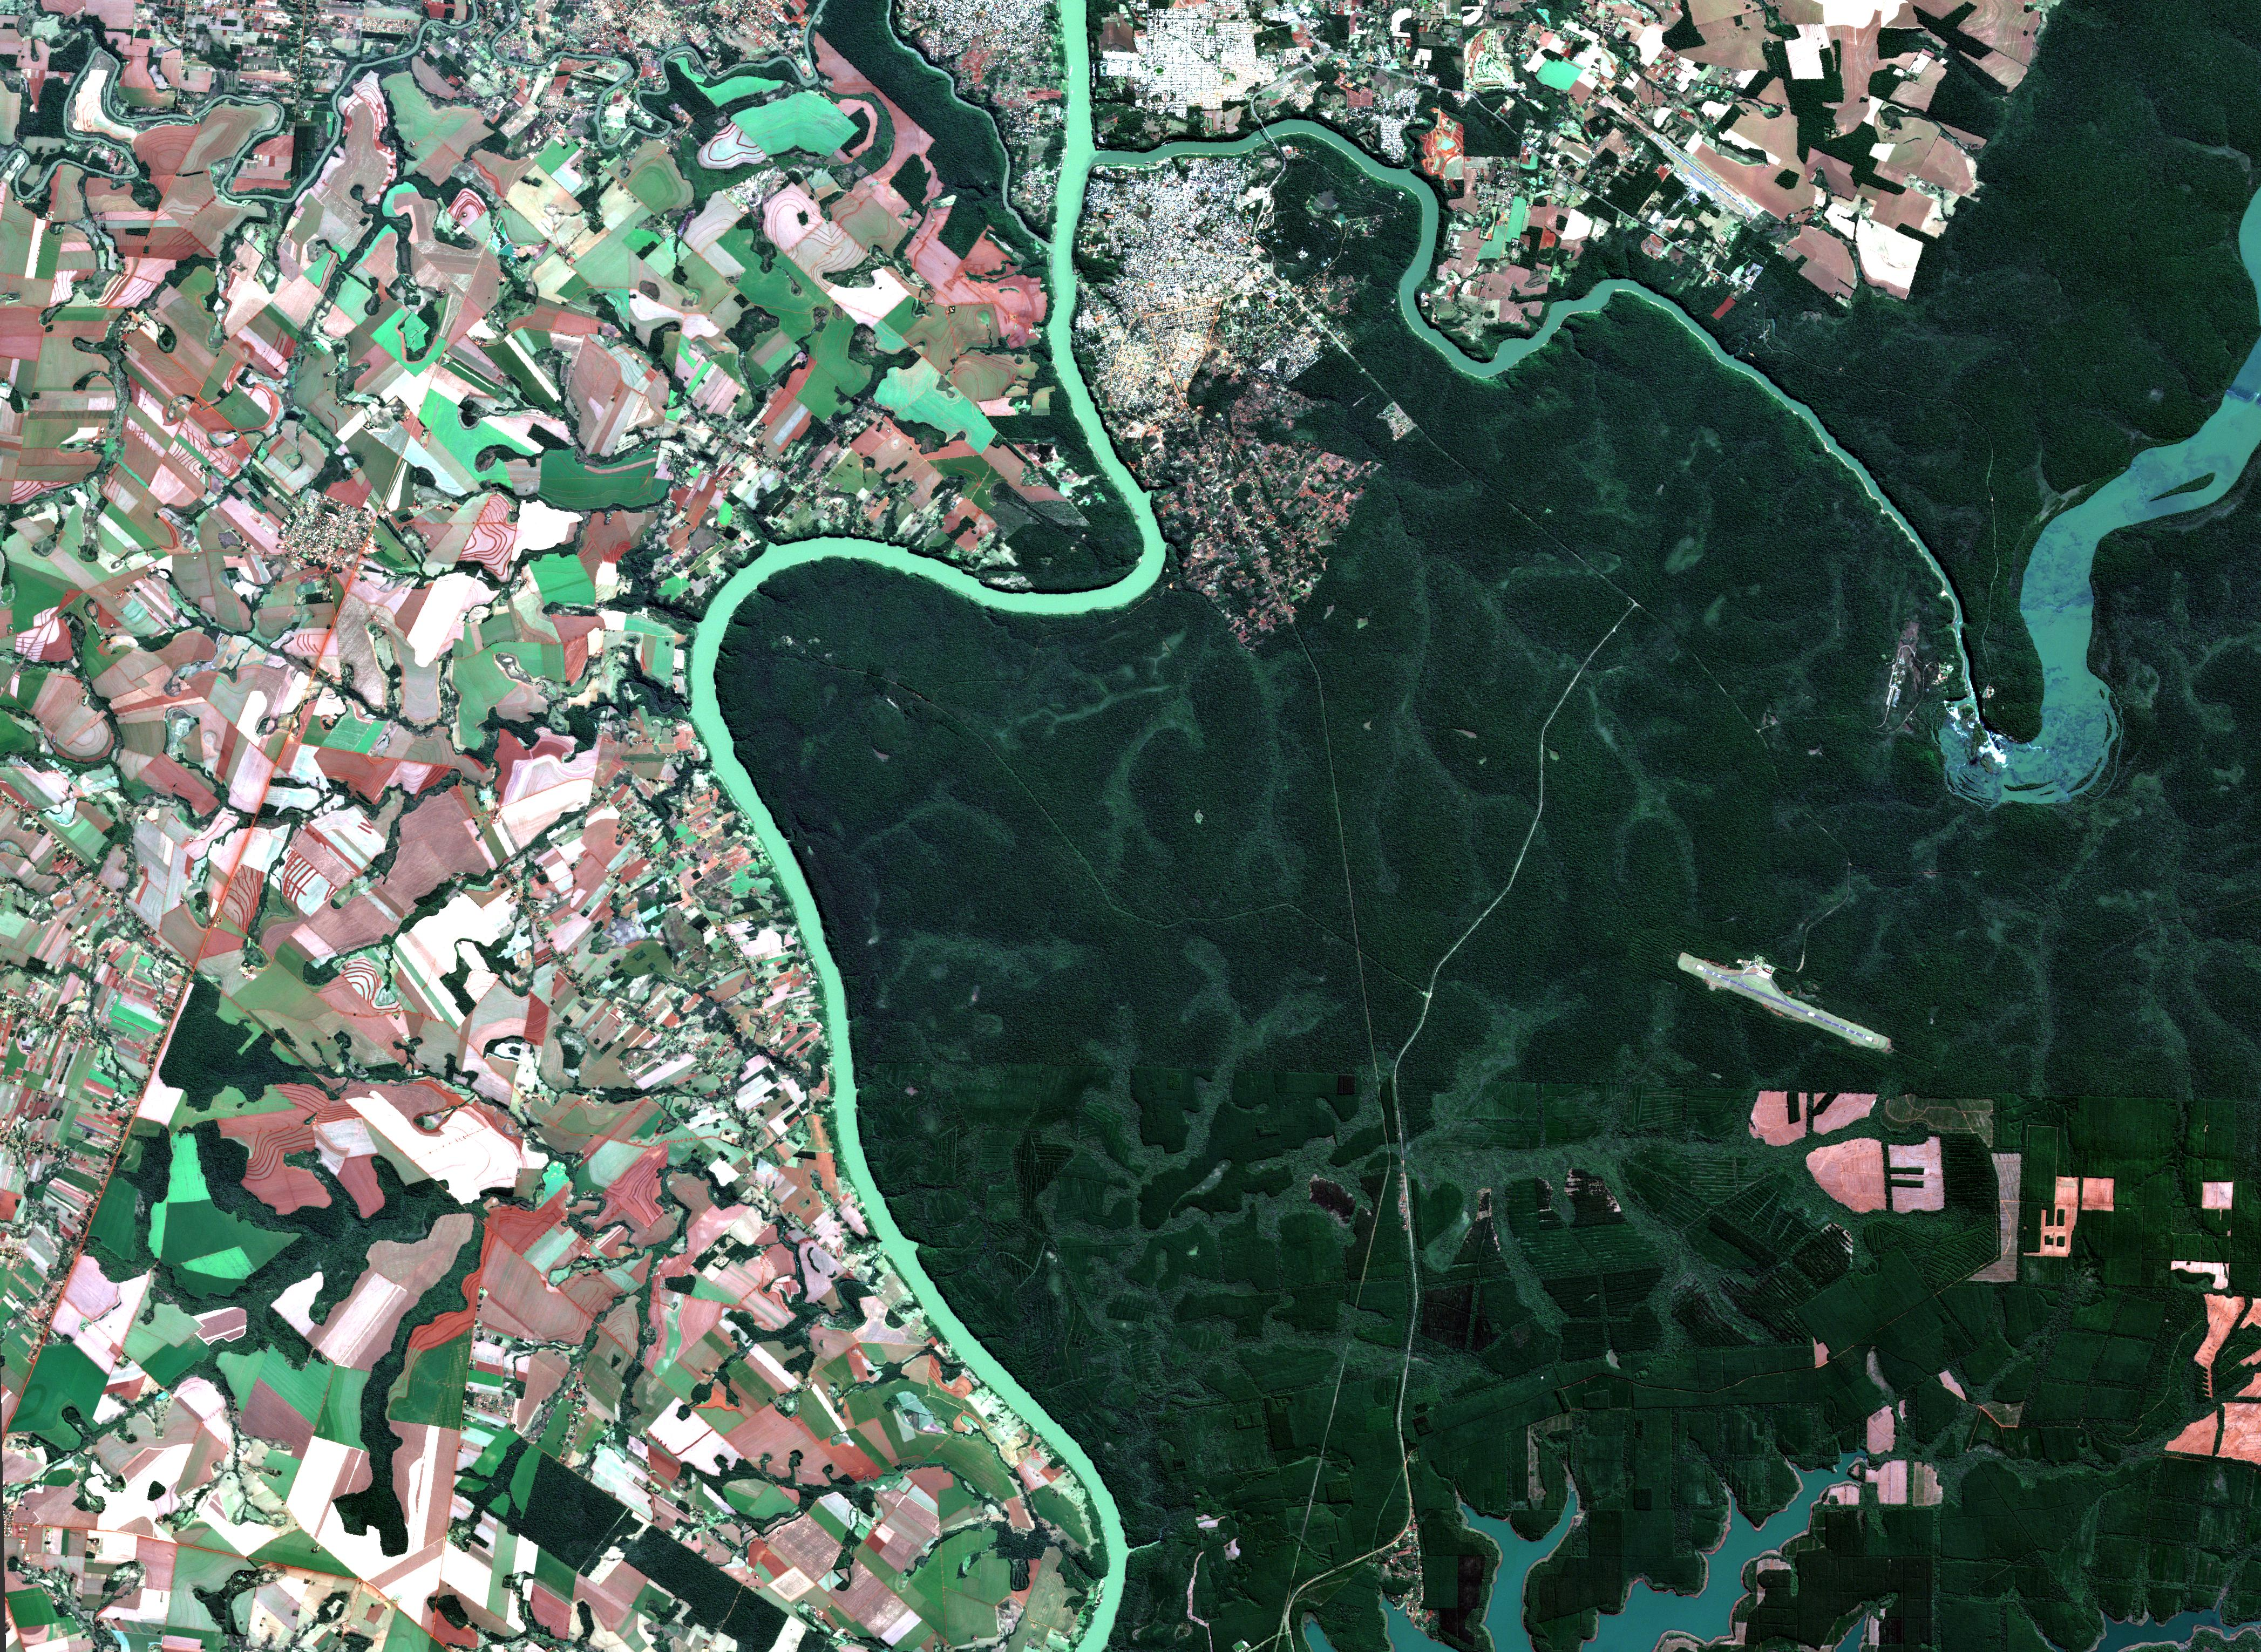
\includegraphics[width=0.6\textwidth]{4-3-2.jpeg}
        \caption{Combinación en color real.}
        \label{4-3-2}
    \end{figure}
\end{frame}
%--- Next Frame ---%

\begin{frame}{\secname : \subsecname}
    \begin{figure}[h!]
        \centering
        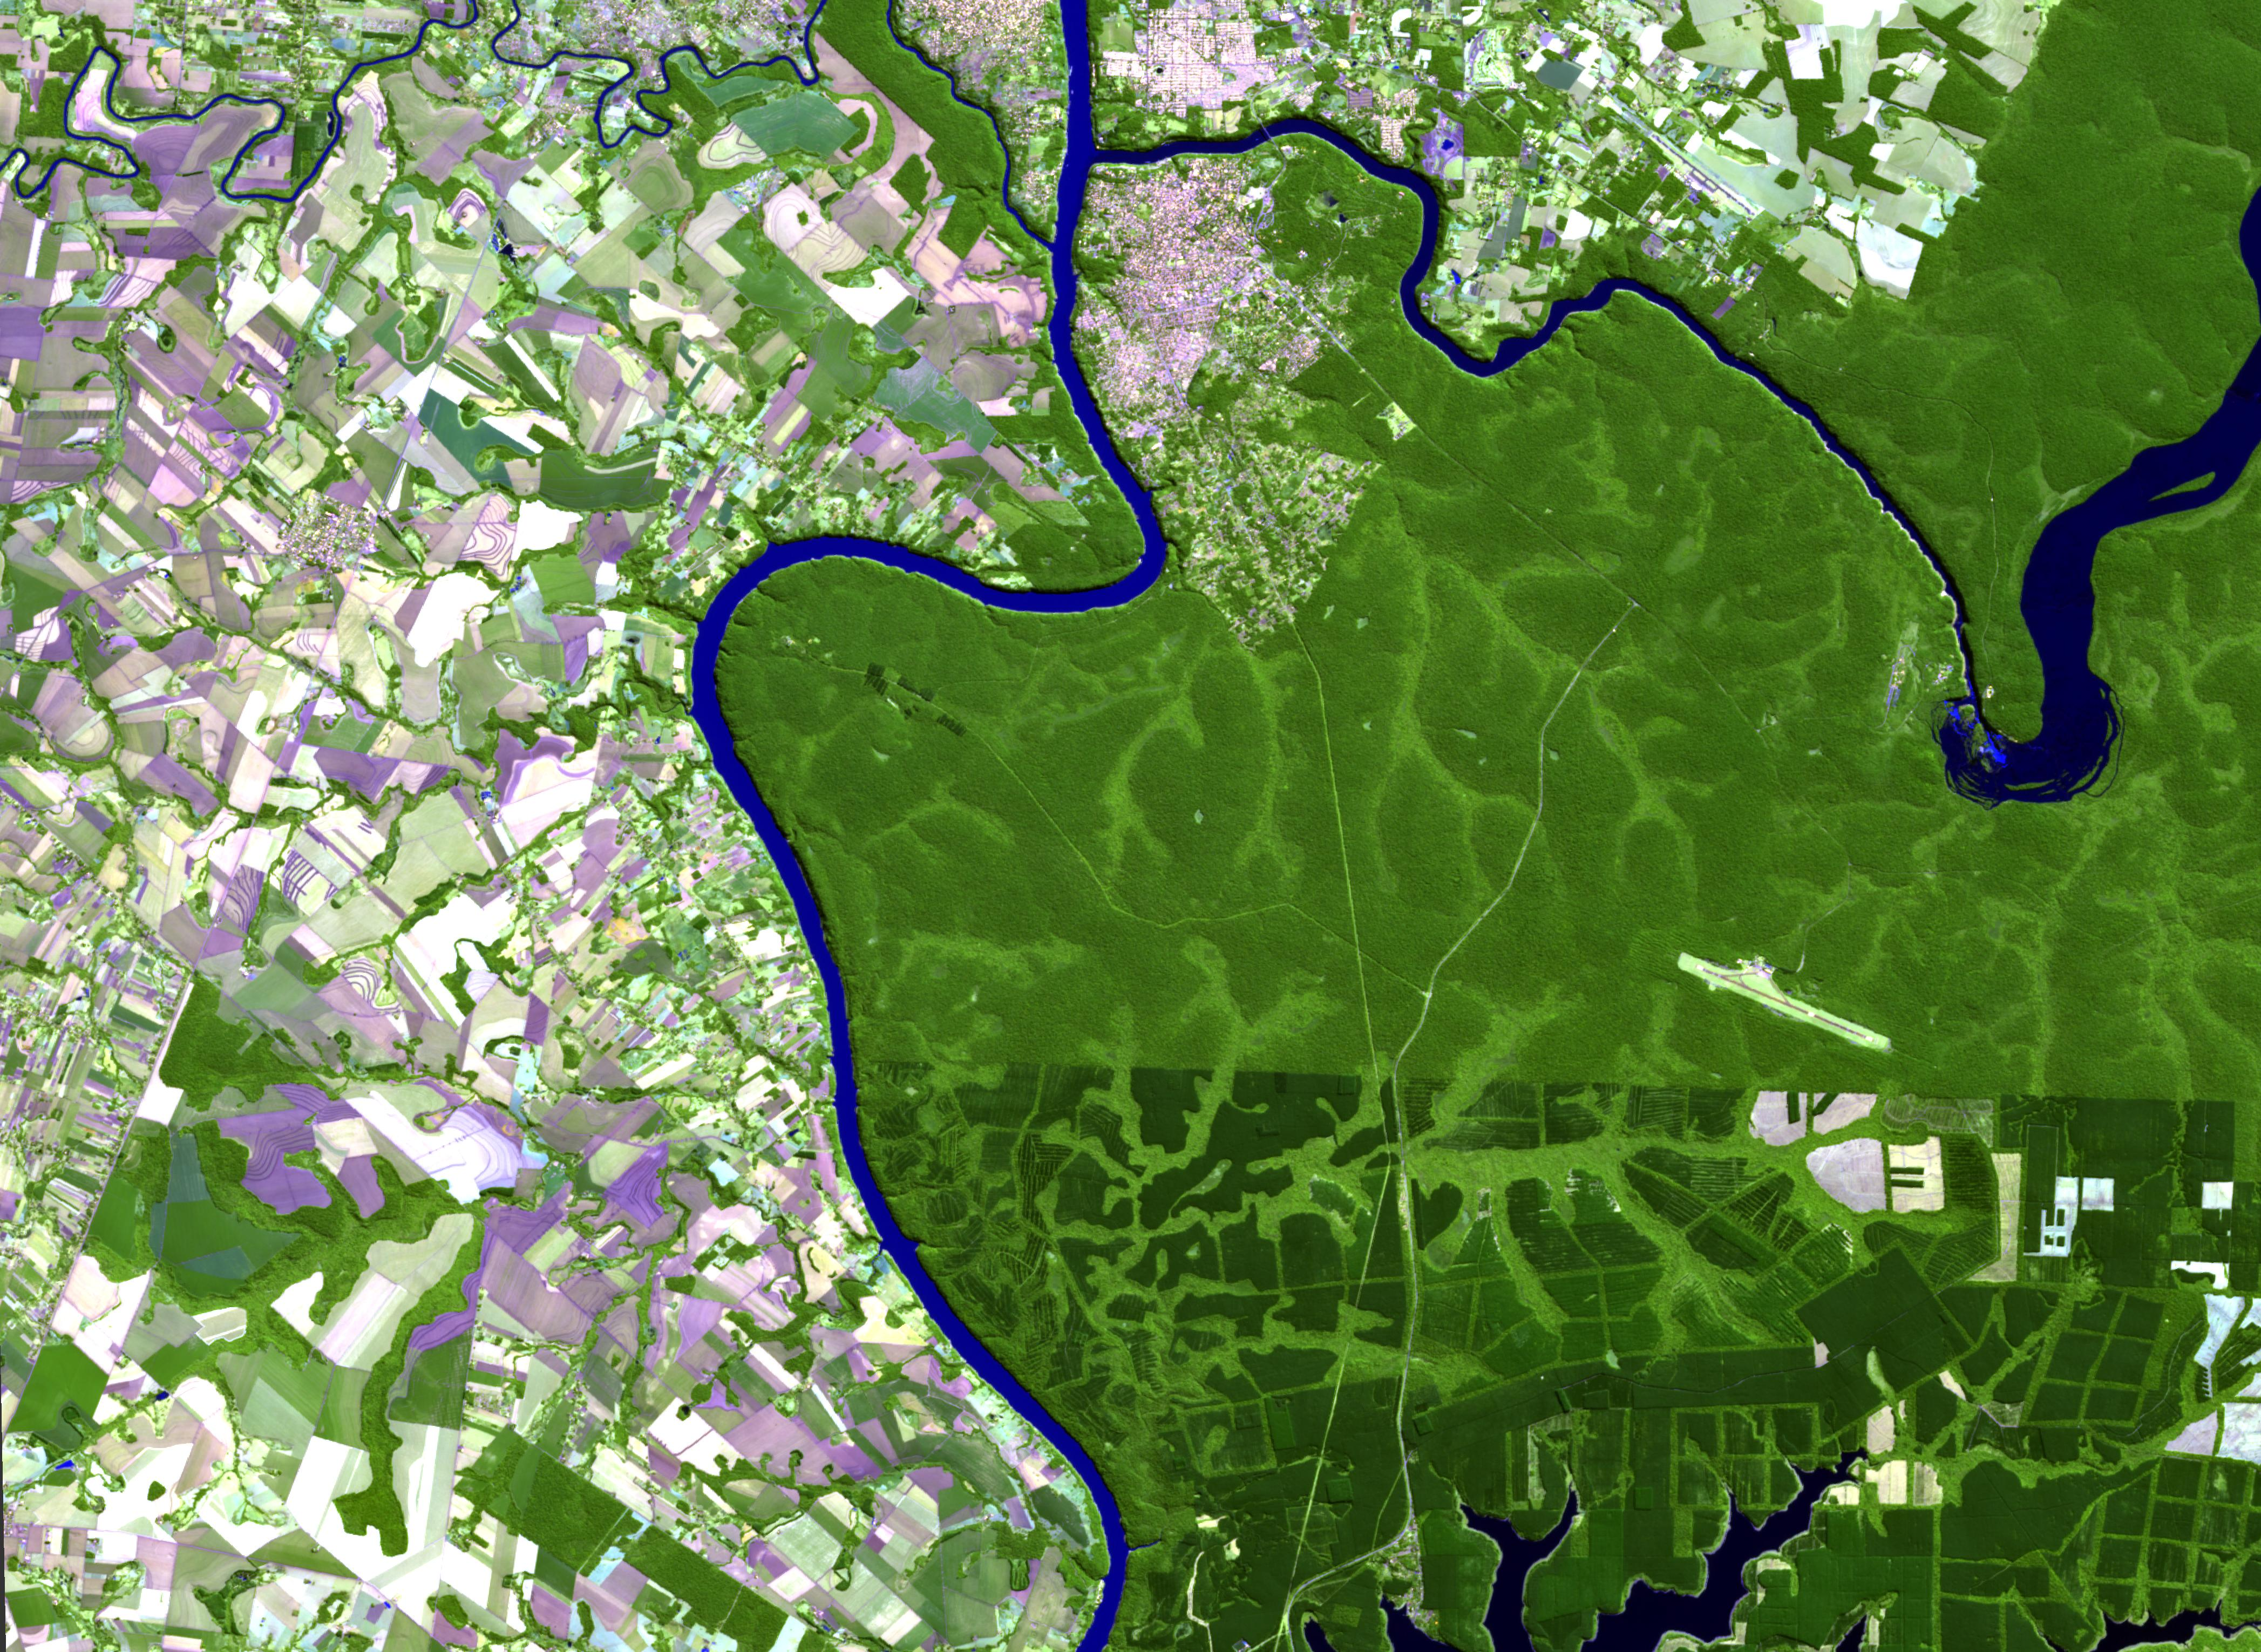
\includegraphics[width=0.6\textwidth]{12-11-4.jpeg}
        \caption{Combinación en falso color - urbano.}
        \label{12-11-4}
    \end{figure}
\end{frame}
%--- Next Frame ---%

\begin{frame}{\secname : \subsecname}
    \begin{figure}[h!]
        \centering
        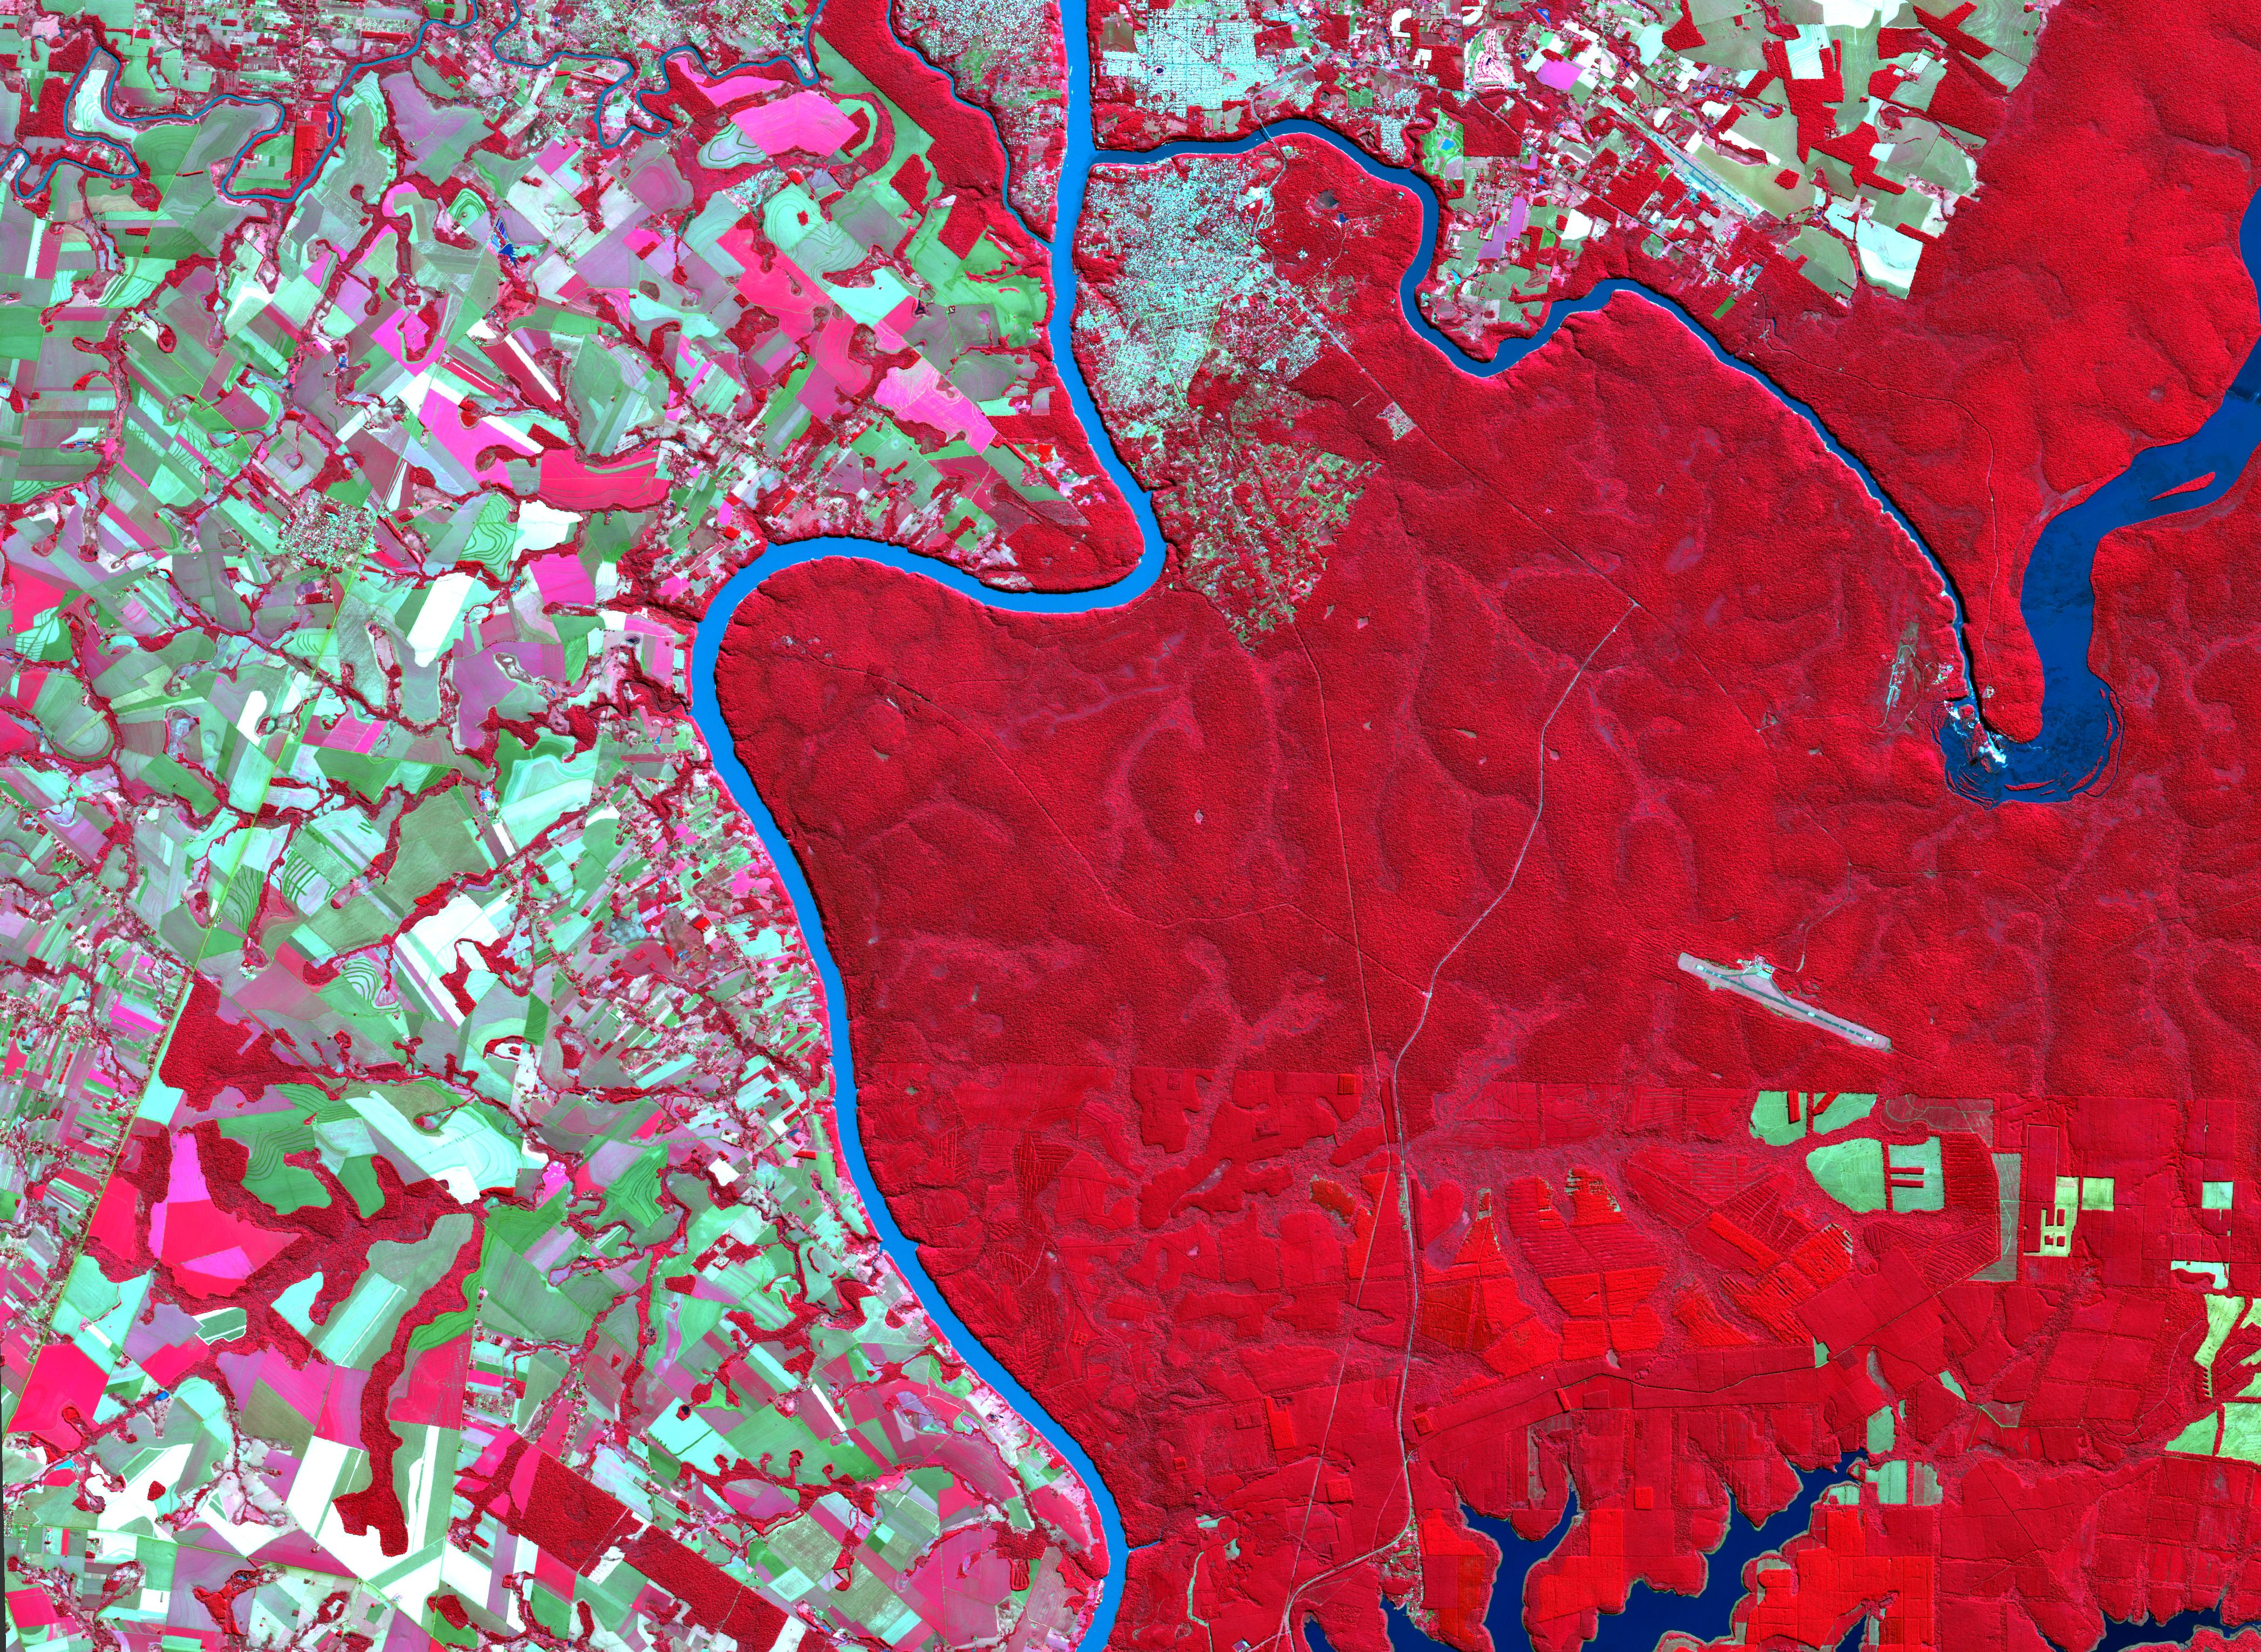
\includegraphics[width=0.6\textwidth]{8-4-3.jpeg}
        \caption{Combinación en infrarrojo color.}
        \label{8-4-3}
    \end{figure}
\end{frame}
%--- Next Frame ---%

\begin{frame}{\secname : \subsecname}
    \begin{figure}[h!]
        \centering
        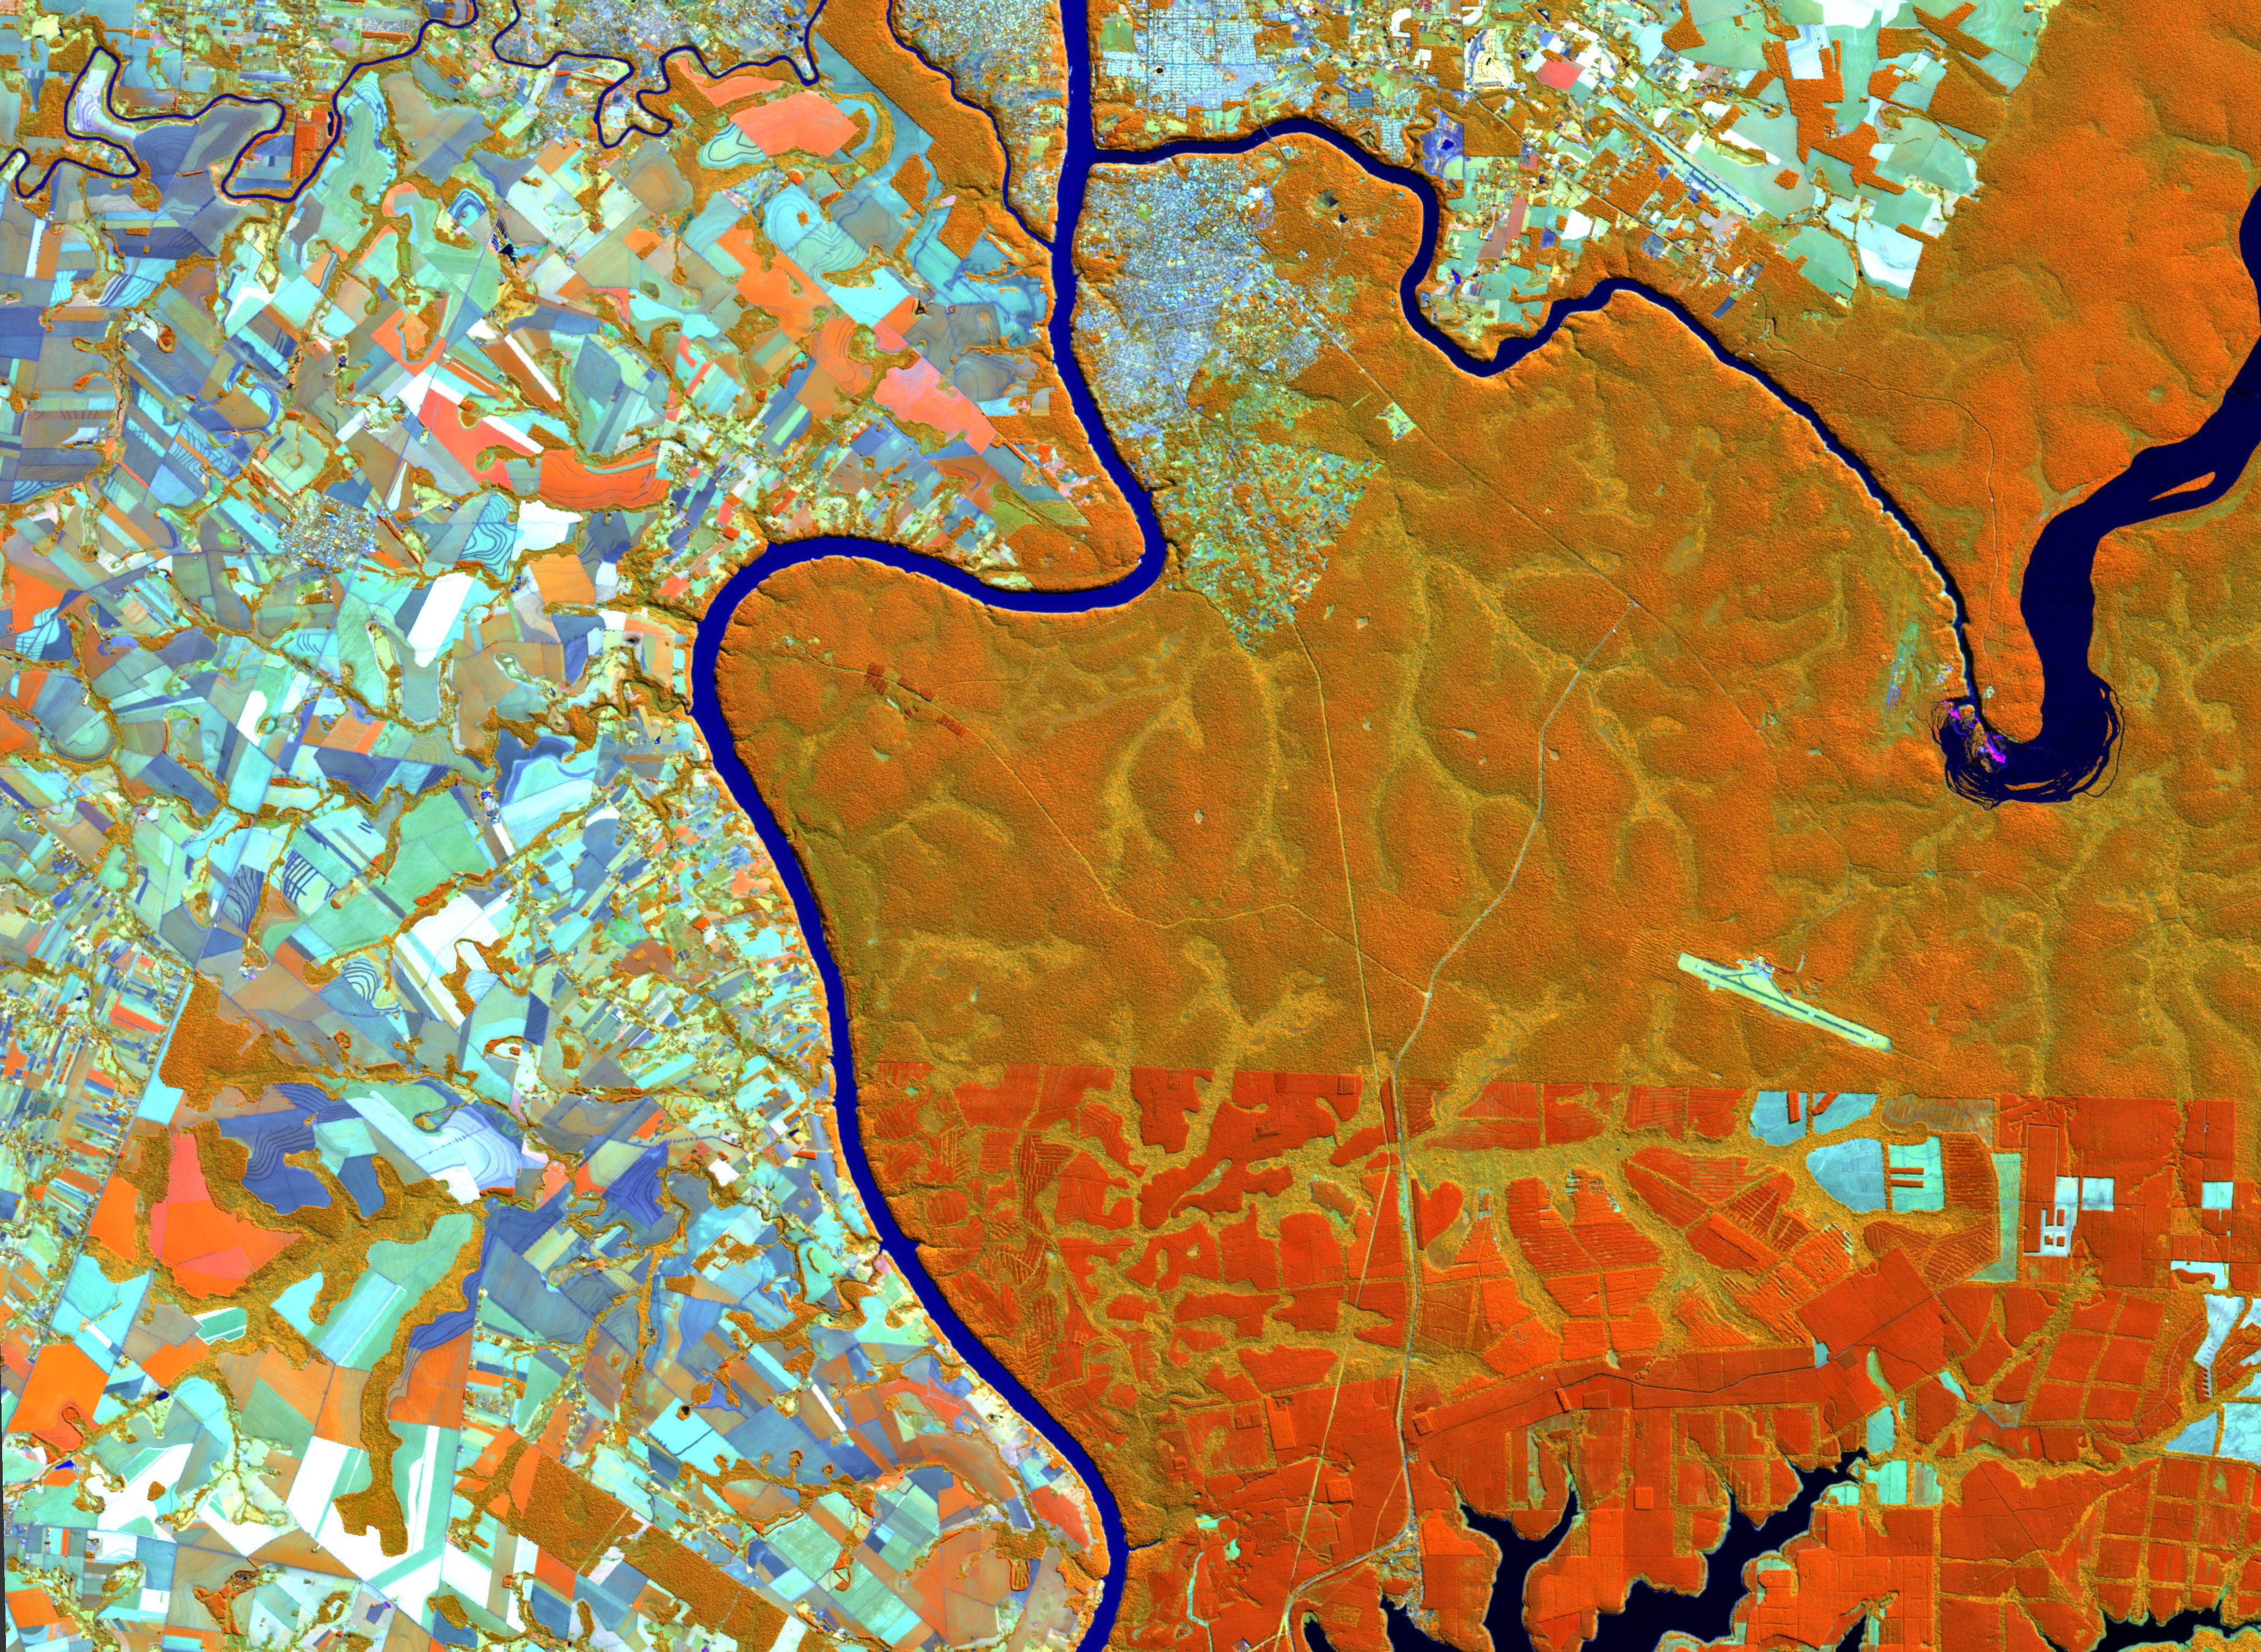
\includegraphics[width=0.6\textwidth]{8-11-4.jpeg}
        \caption{Combinación en falso color - tierra/agua.}
        \label{8-11-4}
    \end{figure}
\end{frame}
%--- Next Frame ---%

\subsection{Actividad}

\begin{frame}{\secname : \subsecname}
    \begin{alertblock}{Combinaciones espectrales}
        Cambio de combinaciones espectrales y medición de áreas incendiadas.
    \end{alertblock}
\end{frame}
%--- Next Frame ---%

\section{Capacitaciones}
\subsection{CONAE}
\begin{frame}{\secname : \subsecname}
    \begin{block}{Areas de capacitación}
    \begin{itemize}
        \item Unidad de educación
        \begin{itemize}
            \item \href{https://2mp.conae.gov.ar}{Proyecto 2Mp}
            \item \href{https://sopi.conae.gov.ar}{Proyecto SoPI}
        \end{itemize}
        \item \href{http://ufs.conae.gov.ar/}{Unidad de formación superior}
        \item \href{http://ig.edu.ar/}{Instituto Gullich}
    \end{itemize}
    \end{block}
\end{frame}
%--- Next Frame ---%

\begin{frame}{\secname : \subsecname}
    Muchas gracias.
\end{frame}
%--- Next Frame ---%


\end{document}
